\documentclass[12pt,number]{IC_fyp}
\usepackage{a4wide,amsmath,amssymb,epsfig, authordate1-4} 
\usepackage{graphicx} % 用于插入图片
\usepackage{atbegshi} % 可以在页面开始时插入内容

\usepackage{float}
% \usepackage[small]{caption}
\usepackage[tight]{subfigure}

\usepackage{xcolor}   % For color control
\usepackage{graphicx} % For images
\usepackage{array}    % For fixed-width columns
\usepackage{booktabs} % For professional-looking tables
\usepackage{caption}  % For caption formatting
\usepackage{tabularx} % For fulfil cell in table
\usepackage{multirow} % For row merge in table
\usepackage{datatool} % For abbreviation table
\usepackage{longtable}% For long table
\usepackage{makecell} % For change line in table
\usepackage[
    colorlinks=true,    % use color instead of boundingbox
]{hyperref}

% Add Imperial Logo
\newlength{\logowidth} \setlength{\logowidth}{70mm}  % width
\newlength{\logopad}   \setlength{\logopad}{0mm}  % space to margin

\AtBeginShipoutFirst{%
  \put(0,0){%
    \parbox[t][\paperheight][t]{\paperwidth}{%
      \vspace*{\logopad} % adjust v-space
      \hspace*{\logopad} % adjust h-space
      
\includegraphics[width=\logowidth]{Figures/IC_New_Logo.pdf} % control width
      \vfill
    }%
  }%
}

\urlstyle{same} % For url front
% \bibliographystyle{authordate2} % 
\floatstyle{plaintop}
\restylefloat{table}

\renewcommand{\listfigurename}{List of Figures}
\renewcommand{\listtablename}{List of Tables}
% \renewcommand{\UrlFont}{\normalfont\itshape} % change to italic url

\DTLnewdb{acronyms}
\DTLnewrow{acronyms}\DTLnewdbentry{acronyms}{abbr}{ILA}\DTLnewdbentry{acronyms}{full}{Inner London Area}
\DTLnewrow{acronyms}\DTLnewdbentry{acronyms}{abbr}{GLA}\DTLnewdbentry{acronyms}{full}{Greater London Area}
\DTLnewrow{acronyms}\DTLnewdbentry{acronyms}{abbr}{ONS}\DTLnewdbentry{acronyms}{full}{Office for National Statistics}
\DTLnewrow{acronyms}\DTLnewdbentry{acronyms}{abbr}{OA}\DTLnewdbentry{acronyms}{full}{Output Area}
\DTLnewrow{acronyms}\DTLnewdbentry{acronyms}{abbr}{LSOA}\DTLnewdbentry{acronyms}{full}{Lower layer Super Output Area}
\DTLnewrow{acronyms}\DTLnewdbentry{acronyms}{abbr}{MSOA}\DTLnewdbentry{acronyms}{full}{Middle layer Super Output Area}
\DTLnewrow{acronyms}\DTLnewdbentry{acronyms}{abbr}{LAD}\DTLnewdbentry{acronyms}{full}{Local Authority District, or Borough in Inner Lonondon Area}

\DTLnewrow{acronyms}\DTLnewdbentry{acronyms}{abbr}{IPF}\DTLnewdbentry{acronyms}{full}{Iterative Proportional Fitting}
\DTLnewrow{acronyms}\DTLnewdbentry{acronyms}{abbr}{MASS--GT}\DTLnewdbentry{acronyms}{full}{Multi-Agent Simulation System for Goods Transport}
\DTLnewrow{acronyms}\DTLnewdbentry{acronyms}{abbr}{MNL}\DTLnewdbentry{acronyms}{full}{Multinomial Logit}

\DTLnewrow{acronyms}\DTLnewdbentry{acronyms}{abbr}{OSM}\DTLnewdbentry{acronyms}{full}{OpenStreetMap}

\DTLnewrow{acronyms}\DTLnewdbentry{acronyms}{abbr}{MF}\DTLnewdbentry{acronyms}{full}{Membership Function}
\DTLnewrow{acronyms}\DTLnewdbentry{acronyms}{abbr}{FIS}\DTLnewdbentry{acronyms}{full}{Fuzzy Inference System}

\DTLnewrow{acronyms}\DTLnewdbentry{acronyms}{abbr}{JSD}\DTLnewdbentry{acronyms}{full}{Jensen-Shannon Distance}
\DTLnewrow{acronyms}\DTLnewdbentry{acronyms}{abbr}{KLD}\DTLnewdbentry{acronyms}{full}{Kullback-Leibler Divergence}
\DTLnewrow{acronyms}\DTLnewdbentry{acronyms}{abbr}{KS Statistic}\DTLnewdbentry{acronyms}{full}{Kolmogorov-Smirnov Statistic}
\DTLnewrow{acronyms}\DTLnewdbentry{acronyms}{abbr}{TVD}\DTLnewdbentry{acronyms}{full}{Total Variation Distance}
\DTLnewrow{acronyms}\DTLnewdbentry{acronyms}{abbr}{VRP}\DTLnewdbentry{acronyms}{full}{Vehicle Routing Problem}


\begin{document}
\hypersetup{
  % colorlinks=true,    % use color instead of boundingbox
  linkcolor=black,    % content and equation color
  citecolor=cyan,     % \shortcite color
  urlcolor=black,       % hyperlink color
  filecolor=black,      
}

% Dissertation Cover
\begin{titlepage}
  \centering
  \vspace*{2cm}
  
  {\Huge\bfseries A Data-Efficient Demand Generation Framework for Multi-Agent Last-Mile Delivery via Fuzzy Logic \par}
  \vspace{1.5cm}
  
  {\Large Yixuan Li\par}
  {\large CID: 06013045\par}
  \vspace{1cm}
  
  {\large Supervised by \\ Professor Panagiotis Angeloudis\par}
  \vspace{0.5cm}
  \vfill
  
  {\large Imperial College London \par}
  {\large Department of Civil and Environmental Engineering \par}
  {\large 29th August, 2025 \par}
\end{titlepage}


% Table of Content
\tableofcontents  % table of contents

\newpage
\listoffigures  % table of figures
\listoftables  % table of tables

\newpage
\title{A Data-Efficient Demand Generation Framework for Multi-Agent Last-Mile Delivery via Fuzzy Logic}

\author{Yixuan Li}

\address{Department of Civil and Environmental Engineering\\
  Imperial College London}

\begin{frontmatter}
  
\begin{abstract}

With the rapid development of e-commerce platforms, last-mile logistics systems face increasing requirements for efficient and environmentally friendly delivery. 
To optimize and validate delivery strategies, last-mile delivery simulation with realistic demand distribution has become essential. 
However, existing methods that generate last-mile delivery demand mainly rely on proprietary data, which is often opaque due to commercial sensitivity, and are limited in scalability and interpretability.
To address these challenges, this study proposes a population-based framework for synthetic order generation. 
The framework first generates a synthetic population using open source datasets and constructs an e-commerce behaviour model based on fuzzy inference, informed by insights from e-commerce industry reports. 
Orders are then generated using the Monte Carlo sampling module. 
For validation, Jensen-Shannon Divergence is employed to quantify the alignment between synthetic orders and real-world distribution. A case study in the Inner London Area demonstrates that as the scale of the synthetic population increases, the distribution of synthetic orders increasingly aligns with the overall purchasing trends in the UK, validating the effectiveness of the proposed inference system. 
The proposed framework exhibits strong scalability, interpretability, and reproducibility, making it suitable for future applications in last-mile delivery simulation and optimization systems.

\end{abstract}

\end{frontmatter}

\section{Introduction}

In recent decades, e-commerce has expanded rapidly, with its market size continuing to grow and accelerating further during the COVID-19 pandemic \cite{eurostat_COVID19impact,ons_COVID19impact}.
According to Statista \shortcite{statista_global_ecommerce24}, global e-commerce revenues will reach approximately 6,477 billion U.S. dollars in 2029. 
In the United Kingdom, revenues are estimated at 185.97 billion U.S. dollars in 2029, with a market penetration of 97.25\% \cite{statista_uk_shopping25_statistic}. 
This trend has directly driven an explosive increase in last-mile delivery demand, making it one of the most critical and challenging components of urban freight systems \cite{statista_global_ecommerce24,review_LR}. 

To improve the efficiency and reliability of last-mile delivery, numerous optimisation algorithms and scheduling strategies have been proposed by academia \cite{review_LR2}, whose effectiveness typically requires validation through simulation experiments. 
Such simulations rely heavily on rich and realistic datasets, with demand data serving as the foundation for building credible models. 
Current data generation methods can be broadly categorised into four types: proportional mapping, discrete choice models, regression models, and hybrid models. 
Specifically, proportional mapping directly allocates macro-level statistics or operational records to individual agents based on population or firm weights; 
discrete choice models decompose the purchasing process into a sequence of decision chains; 
regression models quantify the relationship between purchase behaviour and its influencing factors; 
while hybrid models integrate survey data with statistical inference to enhance model interpretability.

However, these four approaches share three major limitations. 
First, they suffer from limited reproducibility. 
Due to data governance restrictions such as personal privacy protection, order-level datasets containing individual information are difficult to access; moreover, many records involve commercially sensitive information, which firms are reluctant to disclose. Second, most methods rely on a single data source, which may introduce sample bias and compromise the transferability of the results. 
Third, they generally fail to incorporate customer-specific characteristics into the modelling process, leading to low interpretability as well as limited scalability and flexibility for future extensions.

To address these challenges, this study makes two key contributions:

\begin{itemize}
  \item It proposes a comprehensive population-feature-based framework for generating synthetic orders. 
  The framework first constructs a synthetic population using the 2021 UK census data, and then applies a fuzzy inference system (FIS) combined with Monte Carlo sampling to model e-commerce purchasing behaviour and generate synthetic orders.

  \item It demonstrates and validates the applicability of the proposed framework through a case study in the Inner London Area (ILA), where the generated synthetic orders are benchmarked against third-party statistical data for verification.
\end{itemize}

This framework offers several key advantages.
First, instead of relying on proprietary order-level datasets, it exclusively uses publicly available data.
Specifically, the framework employs the 2021 UK census data to generate the synthetic population and integrates multiple open-source reports to construct the FIS-based behaviour model, thereby enhancing reproducibility and transparency. 
Second, the framework leverages multiple data sources and mitigates the risk of sample bias, improving the transferability of results across contexts. 
Third, by explicitly modelling e-commerce customer behaviour through FIS IF-THEN rules, the framework incorporates customer-specific characteristics, leading to improved interpretability as well as greater scalability and flexibility in future extension. 

The remainder of this paper is organised as follows. 
Chapter \ref{sec:literature} reviews existing research on synthetic demand modelling in last-mile delivery simulation, highlighting current methodologies, their applications, and limitations in capturing demographic-driven e-commerce customer behaviours. 
Chapter \ref{sec:data} introduces the details of the spatial granularity and relevant data sources used for constructing the proposed framework. 
Chapter \ref{sec:methodology} presents the proposed framework, including the overall structure, the synthetic population and synthetic order generation method, and the validation and verification procedures applied to ensure the effectiveness of the proposed method. 
Chapter \ref{sec:results} introduces the case study area (ILA), summarises the results, including the sample of the synthetic instances, validation metrics and analysis regards to them, while Chapter \ref{sec:conclusion} concludes the study with a discussion of key findings, implications for last-mile logistics modelling, limitations and potential directions for future research.


\section{Literature Review}
\label{sec:literature}

This section begins with a review of agent-based simulation methods, summarising commonly used demand modelling approaches, including Proportional Mapping, Discrete Choice Models, Regression Models and Behaviour-Structure Hybrid Models.
It then compares their characteristics, applicability, and limitations, providing a theoretical foundation and motivation for the population-feature-based framework proposed in this study.

\subsection{Agent-based Simulation and Demand Modelling in Last-mile Delivery}

Accurate modelling of last-mile delivery is essential for efficient urban logistics planning. 
Currently, extensive research has explored simulation frameworks and logistics functions for last-mile delivery. 

To address the surge in parcel volumes driven by the rapid growth of B2C e-commerce and its resulting pressures on traffic and the environment, Bienzeisler Lasse \shortcite{bienzeisler_matsim2025} proposed a regional agent-based freight simulation framework using MATSim. 
Unlike previous studies that focus on a single city and small-scale samples, this framework leverages real demand data from a parcel delivery company in Hanover, Germany, and extrapolates it to the entire industry, simulating approximately 200,000 deliveries per day. 
The study first constructs a regional transport network and synthetic population covering both roads and public transit, then incorporates multiple carriers and vehicle fleets into the MATSim freight extension, and finally identifies eight typical spatial zones through geographic clustering to enable comparative analysis across urban, suburban, and rural areas.
Michiel de Bok et al. \shortcite{michiel_massGT2025} proposed an agent-based model for urban- and regional-scale freight policy evaluation, called MASS-GT (Multi-Agent Simulation System for Goods Transport). 
The model centers on multi-agents, for example, shippers, carriers, and production/consumption firms, and integrates discrete choice, heuristic scheduling, and network assignment algorithms to connect the full chain: freight generation, vehicle scheduling, road assignment, and emission accounting. 
It enables scenario analysis for various policies, including low-emission zones, road pricing, micro-hubs, and crowdsourcing.
Sebastian Hörl et al. \shortcite{horl_equasim2023} proposed an open-source and reproducible modelling pipeline: starting from public data to generate population and travel demand, then inferring residential parcel demand, and finally using JSprit to solve the time-windowed pickup-and-delivery vehicle routing problem to evaluate the last-mile performance of autonomous delivery robots, demonstrated on the Confluence peninsula in Lyon, France. 

In these studies, demand serves as the input for subsequent simulations, but its generation process is often simplified. 
For example, Bienzeisler Lasse \shortcite{bienzeisler_matsim2025} directly extrapolated actual company micro-demand to the entire industry based on market share, without modelling individual delivery behaviours in detail. 
Michiel de Bok et al. \shortcite{michiel_massGT2025} rely directly on historical travel diaries to generate synthetic demand.
Hörl et al. \shortcite{horl_equasim2023} discretised  annual purchase frequencies into daily parcel counts using a Poisson distribution, focusing on aggregate demand rather than individual delivery features. Other approaches rely directly on historical travel diaries to generate synthetic demand. These simplifications allow large-scale simulations while abstracting away fine-grained details of individual deliveries.


\subsection{Synthetic Order Generation}

At the micro level, existing methods for demand generation can be broadly classified into four categories: proportional mapping, regression models, discrete choice models, and hybrid models.
Related studies and their corresponding data sources and methods are listed in Table \ref{tab:freight_models}.

\begin{table}[htbp]
  \centering
  % \small % use smaller font size
  \caption{Comparison of Methods and Data Sources across Different Simulation Frameworks}
  \label{tab:freight_models}
  \resizebox{\textwidth}{!}{%
  \begin{tabular}{
    >{\centering\arraybackslash}m{3cm} 
    >{\centering\arraybackslash}m{2.8cm} 
    >{\raggedright\arraybackslash}m{4.5cm} 
    >{\centering\arraybackslash}m{4.5cm} 
    >{\centering\arraybackslash}m{5cm}}
  \toprule
  \textbf{Framework} & \textbf{Method} & \textbf{Data Source} & 
  \textbf{Algorithms Idea} & 
  \makecell{\textbf{Applied City \&} \\ \textbf{Use Case}} \\
  \midrule

  \makecell{MATSim-freight \\ Bienzeisler, L. \\ \shortcite{bienzeisler_matsim2025}} & 
  Proportional Mapping & 
  MiD 2017 [58k records] \shortcite{miD2017}; Logistics Services Provider operator data* & 
  Operator data extrapolated based on market share & 
  Germany - Greater Hannover (urban--suburban--rural); unified carrier evaluation, locker coverage estimation \\
  \midrule

  \makecell{MASS-GT \\ de Bok, M. et al. \\ \shortcite{michiel_massGT2025}} & 
  Discrete Choice Model & 
  XML truck trip diaries [2.65 M records] \shortcite{cbs_opendata}; Mobility Panel Netherlands, Online orderings [6k records] \shortcite{MPN_2015} & 
  Ordered Logit assigns frequency (0--4 bins), then expanded to daily count & 
  Netherlands: National-level (Rotterdam, Amsterdam pilot); includes policy modules (crowdsourcing, micro-hubs) \\
  \midrule

  \makecell{Eqasim-based \\ H\"orl \& Puchinger \\ \shortcite{horl_equasim2023}} & 
  Hybrid Models & 
  Survey Achats D\'ecoupl\'es de M\'enages [2k records] \shortcite{ADM_2016} &
  IPF constrains annual e-commerce frequency to occupation, age, and household size margins; Poisson sample daily parcels & 
  France - Lyon Metro Area; used in robotic VRP (Vehicle Routing Problem) scenario analysis \\
  \midrule

  \makecell{LogiTopp \\ Reiffer et al.\\ \shortcite{reiffer_logitopp2023}} & 
  Discrete Choice Model \& Regression Model & 
  Online survey [1k records]*; MiD 2017 [58k records] \shortcite{miD2017} & 
  Three discrete choices (e-commerce participation, order quantity, delivery location) & 
  Germany - Karlsruhe; joint passenger-freight evaluation for locker deployment and failed delivery strategies \\
  \midrule

  \makecell{Spatial ABM \\ Calabr\`o et al.\\ \shortcite{calabro_spatialABM_2023}} & 
  Proportional Mapping & 
  National census statistics (Italian Statistic Institute) \shortcite{istat_dataset} & 
  GIS analysis -- spatially assigning e-commerce demands based on statistics reports & 
  Catania (Southern Italy); compared fragmented door-to-door deliveries with consolidation-based strategies \\
  \midrule

  \makecell{SimMobility \\ Cheng et al. \\ \shortcite{cheng_simMobility2020}} &
  Regression Model & 
  Parcel delivery record [1.7M record]* & 
  Linear regression of parcel demand vs. urbanization, transit, and shopping accessibility & 
  Singapore; used for night-time delivery, time-restricted zones, micro-hub sandbox modeling \\
  
  \bottomrule
  \end{tabular}
}
  \vspace{1mm} \par
  \footnotesize
  {\raggedright
  \textit{Note: Data source with * means the data is proprietary data.}\par}
\end{table}
  

\textit{Proportional Mapping} This approach directly allocates macro-level statistics or operational records to individual agents based on population or firm weights. 
For example, in the MATSim-freight model \cite{bienzeisler_matsim2025}, parcel volumes are estimated as a linear combination of population and firm count and then assigned to the nearest household or firm. 
Similarly, Calabr\`o et al. \shortcite{calabro_spatialABM_2023} spatially allocate e-commerce orders to zones based on national statistics, with residents classified according to age and purchasing frequency.

\textit{Discrete Choice Models} This category decomposes the purchase process into a chain of decisions, such as whether to buy, how many to buy, delivery method and time window. 
These choices are modelled using Binary Logit \cite{reiffer_logitopp2023}, Multinomial Logit (MNL) \cite{reiffer_logitopp2023}, or Ordered Logit \cite{michiel_massGT2025}, producing probability distributions as outputs. 
A representative case is the LogiTopp framework proposed by Reiffer et al. \shortcite{reiffer_logitopp2023}. 
They proposed a decision chain to model the customer behaviour, including modelling e-commerce participation using Binary Logit, and modelling delivery location using the MNL model.
MASS-GT \cite{michiel_massGT2025}, in turn, applies an Ordered Logit to assign shopping frequency (0-4 bins), which is then expanded into daily parcel counts.

\textit{Regression Models} These models quantify the relationship between purchase frequency with its impact factors.
For instance, in the LogiTopp framework \cite{reiffer_logitopp2023}, a Poisson regression was employed to model the purchase behaviour across different ages and occupations.
Similarly, in the SimMobility framework proposed by Cheng et al. \shortcite{cheng_simMobility2020}, Linear regression was used to estimate the parcel demand based on urbanization rate, shopping accessibility and other factors.

\textit{Behaviour-Structure Hybrid Models} 
This approach integrates survey data with statistical inference. 
Typically, annual purchase frequencies are first assigned to households via surveys or Iterative Proportional Fitting (IPF), followed by the use of a Poisson distribution to generate daily parcel volumes. 
Delivery time windows are then inferred from individual activity chains. 
For instance, the Eqasim framework in Lyon \cite{horl_equasim2023} applies a three-dimensional IPF to estimate annual frequencies, a Poisson model to generate daily counts, and extracts at-home windows from activity chains to determine delivery feasibility.

Despite their differences, these four approaches share some major limitations. 
First, they generally require large volumes of detailed data to support reliable parameter estimation and calibration, and many of those sources are proprietary data that hinder the reproducibility, as indicated in Table \ref{tab:freight_models}. 
Second, when training algorithms such as discrete choice models, most models rely on a single data source, which increases the risk of sample bias and limits flexibility for future extensions. 
In addition, they are often criticised for their limited intuitiveness and interpretability.


\subsection{Research Gap}

In last-mile logistics demand modelling, micro-level demand generation constitutes the initial step and serves as a critical component of both algorithms and simulation frameworks. 
A more realistic representation of real-world demand can, to a certain extent, ensure the transferability and validity of the overall simulation system. 
However, existing studies often rely heavily on large volumes of real-world data. 
In practice, data scarcity and privacy constraints pose significant challenges to such approaches. 
Hence, there is an urgent need for a more flexible and human-centred methodology that can reduce data dependency while capturing uncertainty and improving model applicability.

Moreover, current methods generally fail to adequately account for consumer heterogeneity, such as demographic characteristics (e.g., gender, age) and behavioural preferences. 
At the same time, the reliance on single-source datasets limits the robustness and applicability of these models. 
Therefore, it is necessary to develop a new modelling framework that addresses these limitations:
\begin{itemize}
  \item \textbf{Enhanced reproducibility and privacy protection:} Utilise open data sources to protect privacy, reducing reliance on proprietary or commercially sensitive datasets. 
  \item \textbf{Improved robustness and transferability:} Leverage multi-source data to mitigate sample bias, enhancing scalability and applicability across different contexts.  
  \item \textbf{Better representation of consumer heterogeneity:} Explicitly model customer-specific characteristics, including demographic attributes, thereby increasing interpretability.
\end{itemize}



\section{Data}
\label{sec:data}

This section describes the datasets used in this study, which primarily include the 2021 UK census data for generating the synthetic population, as well as industry reports and academic literature on online shopping behaviour for constructing the FIS and generating synthetic orders.



\subsection{United Kingdom Census Data}
\subsubsection{Data Granularity}

The United Kingdom Population Census is a nationwide survey conducted every ten years to collect comprehensive information about every person and household, with the most recent taking place in 2021 for England, Wales, and Northern Ireland \cite{uk_census}.
It is administered by the Office for National Statistics (ONS) in England and Wales, the National Records of Scotland, and the Northern Ireland Statistics and Research Agency. 
The census provides an accurate snapshot of the population's size, structure, and detailed demographic features.

The statistical summary of census data is released at multiple levels of spatial resolution to balance the analytical value and confidentiality.
The smallest available geography is the Output Areas (OAs), and is followed by Lower layer Super Output Areas (LSOAs), Middle layer Super Output Areas (MSOAs) \cite{census_geographies}. 
Additionally, a statistical summary of Local Authority District (LAD) is also provided by the UK Data Service \shortcite{census_lad}.
The granularity of OA, LSOA and MSOA makes up the different levels of the census statistical geographies, and their features are compared in Table \ref{tab:geo_levels}.

\begin{table}[h]
  \centering
  \caption{Geography Levels Comparison}
  \label{tab:geo_levels}
  \begin{tabular}{c c c c m{3.8cm}}
      \toprule
      \textbf{Geography} & \textbf{Persons} & \textbf{Households} & \textbf{Units in ILA} & \textbf{Illustration} \\
      \midrule
      OA   & 100 -- 625 &  40 -- 250  & 10356   & \includegraphics[width=3.5cm]{Figures/oa.pdf} \\
      LSOA* & 1,000 -- 3,000 & 400 -- 1,200  & 1983 & \includegraphics[width=3.5cm]{Figures/lsoa.pdf} \\
      MSOA & 5,000 -- 15,000 & 2,000 -- 6,000   & 404 & 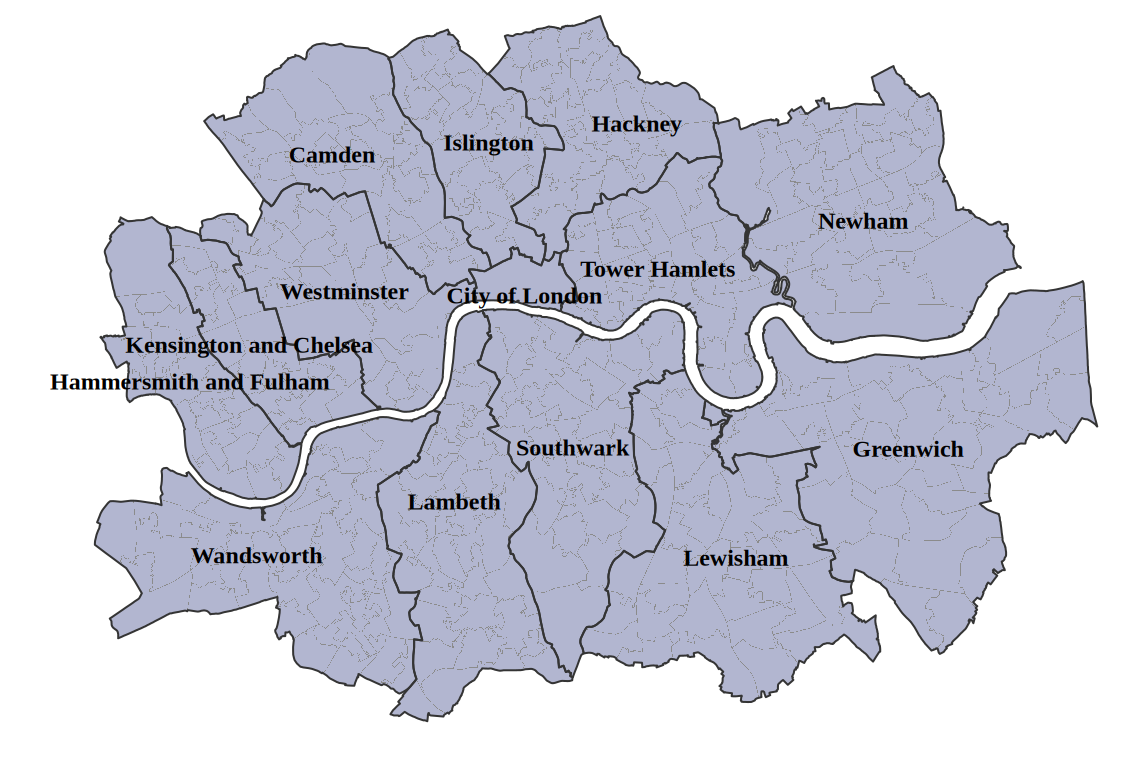
\includegraphics[width=3.5cm]{Figures/msoa.pdf} \\
      LAD  & 8,000 -- 350,000 &  5,000 -- 140,000   & 14 & 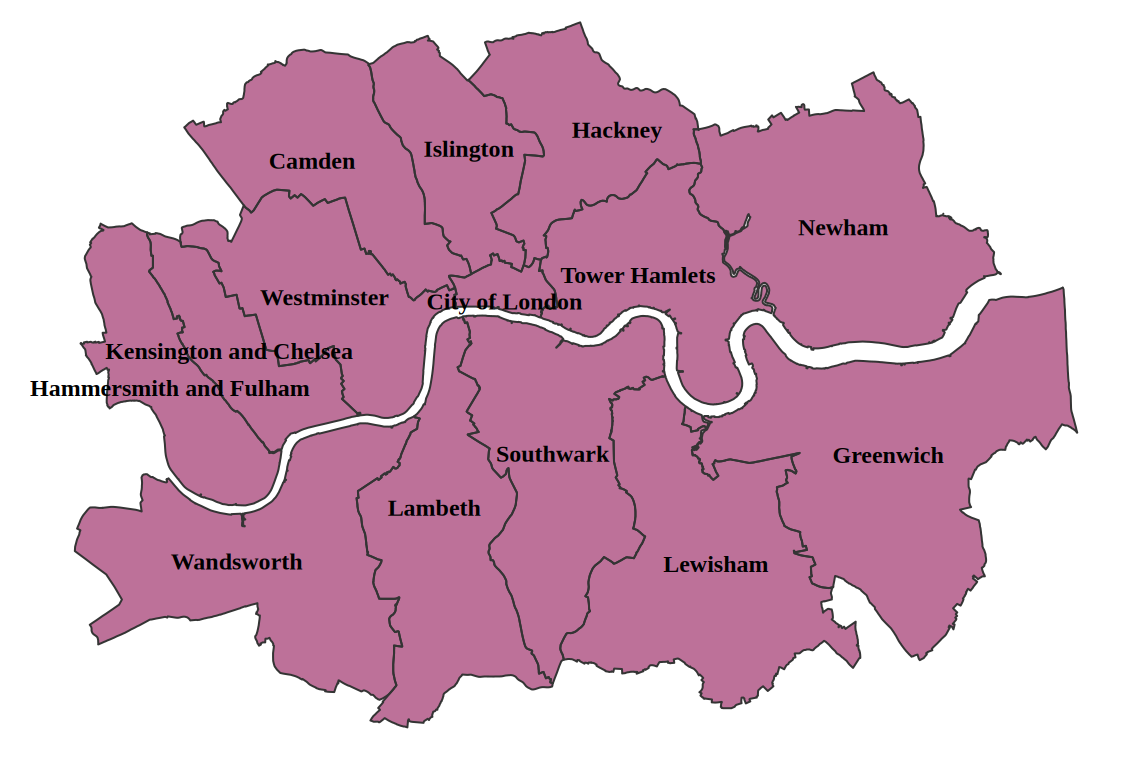
\includegraphics[width=3.5cm]{Figures/lad.pdf} \\
      \bottomrule
  \end{tabular}
  \vspace{1mm} \par
  \raggedright{\textit{Note: Geography Level with * is the final synthetic population level.}}
\end{table}

To achieve a more granular and realistic population, smaller geography units are preferred.
However, given the varying availability of demographic feature statistics across different geography levels, the LSOA level is ultimately selected as the optimal geography level for synthetic population generation.

\subsubsection{Census Data Products}
The census results are released in different formats, including 1) Aggregate Statistics and 2) Microdata Samples.

The Aggregate Statistics, provided by UK Data Service \shortcite{ukDataService} include counts and percentages for specific categories (e.g., age, sex) at various geographies. 
As for microdata samples, for security and confidentiality considerations, micro census sample data is released in different formats and levels of access, including:

\begin{itemize}
  \item \textbf{Public Microdata Sample} Covers ~1\% of the population (604,351 persons). It contains 19 variables and a low level of detail \shortcite{ONS_public_microdata}.
  \item \textbf{Safeguarded Microdata Sample} It includes two formats of data sample, individual microdata sample (5\%, 3,021,455 persons \shortcite{ONS_safeguarded_individual}) and household microdata sample (1\%, 263,729 households and 606,210 persons \shortcite{ONS_safeguarded_household}) with richer variables and smaller geographies.
  This data requires UK Data Service registration.
  \item \textbf{Secure Microdata Sample} Similar to safeguarded microdata, secure microdata also includes two formats of data sample, but with 10\% of households or individual persons. 
  It contains the most detailed variables and a high level of detail.
  However, this data is available only via the ONS Secure Research Service.
\end{itemize}

The comparison of different microdata sample products is shown in Table \ref{tab:microdata_products}. 
In this study, we focus on individual-level e-commerce behaviour.
Considering both the data detail level and accessibility, the safeguarded-level individual microdata sample is selected as the original data sample for subsequent data curation, as highlighted in Table \ref{tab:microdata_products}.


\begin{table}
  \centering
  \caption{Comparison of Microdata Sample Products}
  \label{tab:microdata_products}
  \begin{tabular}{c c c c c}
    \toprule
    \textbf{Product Type} & \textbf{Level} & \textbf{Sample Rate} & \textbf{Category}  & \textbf{Availability} \\
    \midrule
    Public & Person & 1\% & 19 & Open Access \\
    \textbf{Safeguarded*} & Person & 5\% & 87 & Registration \\
    Safeguarded & Household & 1\% & 56 & Request Access \\
    Secure & Person & 10\% & 189 & Limited \\
    Secure & Household & 5\% & 194 & Limited \\
    \bottomrule
  \end{tabular}
  \vspace{1mm} \par
  \textit{Note: Product with * is the final microdata for subsequent steps.}
\end{table}



\subsection{E-commerce Reports}
\label{sec:e-commerce_data}

Since the development of online shopping platforms, as well as the e-commerce change after COVID-19, many studies have found the relationship between the socio-demographic characteristics of e-commerce customers and their shopping behaviour. 
For example, according to Eurostat and findings from Colaço et al. \shortcite{colaco_ecommerce_2021}, younger people buy online more often compared to older people.
According to statistics from Amazon \shortcite{amazon_ecommerce_statistics25} and Kráľová et al.\shortcite{Kráľová2025}, statistically significant gender differences existed in the increase in online shopping frequency and order category.
Besides, research shows that household income \cite{cheng_simMobility2020}, level of education \cite{colaco_ecommerce_2021}, and other demographic customer features also impact the online shopping preferences.

To model the e-commerce behaviour in the UK, multiple sources were used, including research articles, industry reports, third-party statistics, and the annual report of online shopping platforms, as summarised in Table \ref{tab:uk_ecommerce_sources}.

% Jenson-Shannon Divergence of Synthetic Order Customer
\begin{longtable}{c p{5.5cm} c p{5cm}}
  \caption{Data Sources of the E-commerce Industry
  \label{tab:uk_ecommerce_sources}} \\
  \toprule
  \textbf{Type} & \textbf{Title} & \textbf{Author} & \textbf{Key Topics} \\
  \midrule
  \endfirsthead
  
  \multicolumn{4}{l}{\textit{Continuation of Table \ref{tab:uk_ecommerce_sources}}}\\
  \toprule
  \textbf{Type} & \textbf{Title} & \textbf{Author} & \textbf{Key Topics} \\
  \midrule
  \endhead
  
  \midrule
  \multicolumn{4}{r}{\textit{Continued on next page}} \\
  \endfoot
  
  \bottomrule
  \endlastfoot

  % ------------------ seeds 0-2 ------------------
  Article & Gender Differences in Consumer behaviour Stemming from the Dynamic Growth of E-Commerce \shortcite{Kráľová2025} & 
  \makecell{Kráľová et al.} & 
  Gender \& Category / Spending Amount (European Survey) 
  \\ 
  Article & Exploring the Relationship between Locational and Household Characteristics and E-Commerce Home Delivery Demand \shortcite{cheng_simMobility2020} & 
  Cheng et al. & 
  Household attributes: Age \& Income 
  \\ 
  Article & Exploring the Interactions between Online Shopping, In-Store Shopping, and Weekly Travel Behavior using a 7-Day Shopping Survey in Lisbon, Portugal \shortcite{colaco_ecommerce_2021} & Colaço et al. & Online-shopping preference \& Level of education
  \\ 
  \midrule
  Report & E-commerce Evolution in Europe: Market Trends \& Consumer Behaviour \shortcite{evalueserve_europe25} & Evalueserve & Country-level Penetration, Category Distribution 
  \\ 
  Report & Descartes 2nd Annual Home Delivery Sustainability Study \shortcite{descartes_euro_consumer23} & \makecell{Descartes \\ Group} & Delivery Time Expectations, Sustainability Preferences 
  \\ 
  Report & E-commerce in the United Kingdom (UK) 2023 \shortcite{statista_uk_ecommerce23_survey} & Statista & Purchase Characteristics and customer features: Willingness, Frequency, Category \& Sex, Age 
  \\
  Report & Online Shopping Behaviour in the United Kingdom (UK) \shortcite{statista_uk_shopping25_statistic} & Statista & Consumer Habits, Online Shopping Attitudes; Category Distribution
  \\ 
  Report & Online Grocery Shopping in the United Kingdom (UK) \shortcite{statista_uk_grocery24_statistic} & Statista & Online-grocery trend; Consumer Habits 
  \\ 
  Report & E-commerce in the United Kingdom (UK) \shortcite{statista_uk_ecommerce24_statistic} & Statista & E-commerce user trend; Retail sales trend; Most popular categories
  \\
  Report & E-commerce Statistics for Individuals \shortcite{eurostat_euro_statistics25} & Eurostat & Customer Features: Age, Purchase Frequency 
  \\
  Report & Amazon Statistics: Key Numbers and Fun Facts \shortcite{amazon_ecommerce_statistics25} & \makecell{Amazon \\ Scout} & E-commerce Trend; Amazon Customer Demographics (Age) \& Top Products
  \\
\end{longtable}

% \begin{table}
%   \centering
%   \caption{Data Sources of UK E-commerce Industry}
%   \label{tab:uk_ecommerce_sources}
%   \begin{tabularx}{\textwidth}{c X c p{5cm}}
%     \toprule
%     \textbf{Type} & \textbf{Title} & \textbf{Author} & \textbf{Key Topics} 
%     \\
%     \midrule
%     Article & Gender Differences in Consumer behaviour Stemming from the Dynamic Growth of E-Commerce \shortcite{Kráľová2025} & 
%     \makecell{Kráľová \& \\ Col.} & 
%     Gender \& Category / Spending Amount (European Survey) 
%     \\ 
%     Article & Exploring the Relationship between Locational and Household Characteristics and E-Commerce Home Delivery Demand \shortcite{cheng_simMobility2020} & 
%     Cheng et al. & 
%     Household attributes: Age \& Income 
%     \\ 
%     Article & Exploring the Interactions between Online Shopping, In-Store Shopping, and Weekly Travel Behavior using a 7-Day Shopping Survey in Lisbon, Portugal \shortcite{colaco_ecommerce_2021} & Colaço et al. & Online-shopping preference \& Level of education
%     \\ 
%     \midrule
%     Report & E-commerce Evolution in Europe: Market Trends \& Consumer Behaviour \shortcite{evalueserve_europe25} & Evalueserve & Country-level Penetration, Category Distribution 
%     \\ 
%     Report & Descartes 2nd Annual Home Delivery Sustainability Study \shortcite{descartes_euro_consumer23} & \makecell{Descartes \\ Group} & Delivery Time Expectations, Sustainability Preferences 
%     \\ 
%     Report & E-commerce in the United Kingdom (UK) 2023 \shortcite{statista_uk_ecommerce23_survey} & Statista & Purchase Characteristics $\times$ customer features: Willingness, Frequency, Category \& Sex, Age 
%     \\
%     Report & Online Shopping Behaviour in the United Kingdom (UK) \shortcite{statista_uk_shopping25_statistic} & Statista & Consumer Habits, Online Shopping Attitudes; Category Distribution
%     \\ 
%     Report & Online Grocery Shopping in the United Kingdom (UK) \shortcite{statista_uk_grocery24_statistic} & Statista & Online-grocery trend; Consumer Habits 
%     \\ 
%     Report & E-commerce in the United Kingdom (UK) \shortcite{statista_uk_ecommerce24_statistic} & Statista & E-commerce user trend; Retail sales trend; Most popular categories
%     \\
%     Report & E-commerce Statistics for Individuals \shortcite{eurostat_euro_statistics25} & Eurostat & Customer Features: Age, Purchase Frequency 
%     \\
%     Report & Amazon Statistics: Key Numbers and Fun Facts \shortcite{amazon_ecommerce_statistics25} & \makecell{Amazon \\ Scout} & Ecommerce Trend; Amazon Customer Demographics (Age) \& Top Products
%     \\
%     \bottomrule
%   \end{tabularx}
% \end{table}


In this study, synthetic orders are generated based on population demographic characteristics (e.g., age, sex, employment, etc.). Therefore, it is essential to model the e-commerce behaviour as a function of based on these demographic attributes.
Among the sources listed in Table \ref{tab:uk_ecommerce_sources}, those containing customer demographic attributes can be employed to identify behavioural patterns or shopping preferences associated with specific population types, such as findings from Cheng et al. \shortcite{cheng_simMobility2020},  customer-related reports from Statista, \textit{E-Commerce in the United Kingdom (UK)} \shortcite{statista_uk_ecommerce23_survey}, Amazon statistics \shortcite{amazon_ecommerce_statistics25}, Eurostat report \shortcite{eurostat_euro_statistics25}. 



Conversely, sources such as \textit{Online Shopping Behaviour in the United Kingdom (UK)} \shortcite{statista_uk_shopping25_statistic} and \textit{Online Grocery Shopping in the
United Kingdom (UK)} \shortcite{statista_uk_grocery24_statistic}, which provides only e-commerce features without customer behavioural information, such as order category distribution, can serve to validate the generated synthetic orders, as detailed in Section \ref{sec:method_order_val}.


\section{Methodology}
\label{sec:methodology}

\subsection{Framework Structure}

The proposed methodology consists of three main modules: (1) synthetic population generation, (2) fuzzy logic-based e-commerce behaviour modelling, and (3) synthetic order generation derived from synthetic population.
The generated synthetic orders are followed by a validation process.
The framework proposed in this study is summarised in Figure \ref{fig:study_framework}, illustrating its main components and their interactions.

\begin{figure}[htbp]
  \centering
  \includegraphics[width=0.9\textwidth]{Figures/study_framework_portrait.pdf}
  \caption{Framework Components and Structure}
  \label{fig:study_framework}
\end{figure}

Section \ref{sec:syn_pop} introduces the synthetic population generation method based on IPF, which constructs a representative population reflecting the demographic characteristics of the study area. 
Section \ref{sec:syn_ord} first presents the construction of the shopping preference model based on FIS, which captures customer purchase behavior in the e-commerce context. 
Subsequently, Section \ref{sec:syn_ord_gen} introduces the synthetic order generation process, where Monte Carlo (MC) sampling with different assumed distributions is employed to instantiate e-commerce customer purchase decisions and produce realistic synthetic orders.

\subsection{Synthetic Population}
\label{sec:syn_pop}
\subsubsection{Iterative Proportional Fitting}

The first stage employs IPF to reconcile differences between sample microdata and aggregate census constraints. 
The process takes the following two as input: 

\textbf{(1) Census microdata:} a sample dataset of UK individuals or households, containing attributes such as age, gender, education, and income.
In this study, safeguarded-person level microdata was chosen, as highlighted in Table \ref{tab:microdata_products}.
Considering the subsequent steps of e-commerce behaviour modelling, only potentially relevant features were selected, generalised into broader categories and recoded, as summarised in Table \ref{tab:synpopfeature}.

\begin{table}[htbp]
  \centering
  \caption{Synthetic Population Feature and Encoding Scheme}
  \label{tab:synpopfeature}
  \begin{tabularx}{\textwidth}{c X}
    \toprule
    \textbf{Feature Name} & \textbf{Values}
    \\
    \midrule
    Age & 0 = 0--15,\; 1 = 16--29,\; 2 = 30--49,\; 3 = 50+ 
    \\
    Sex & 0 = Female,\; 1 = Male 
    \\
    Marital Status & 0 = Single,\; 1 = Married/Registered Same-sex,\; 2 = Separated/Divorced/Widowed 
    \\
    Economic Activity & 0 = Employed,\; 1 = Unemployed,\; 2 = Inactive 
    \\
    Ethnic Group & 0 = Asian,\; 1 = Black,\; 2 = Mixed,\; 3 = White,\; 4 = Other 
    \\
    Number of Cars and Vans & 0 = No car/van,\; 1 = 1 car/van,\; 2 = 2 cars/vans,\; 3 = 3 or more cars/vans 
    \\
    Approximated Social Grade & 0 = AB,\; 1 = C1,\; 2 = C2,\; 3 = DE 
    \\
    \bottomrule
  \end{tabularx}
\end{table}

\textbf{(2) Aggregate constraints:} marginal distribution for each attribute category at aspecific geography level.
In this study, the LSOA level of aggregate constraints is chosen, as highlighted in Table \ref{tab:geo_levels}.
The level of aggregated constraints will determine the geography level of the synthetic population.

\begin{figure}[htbp]
  \centering
  \includegraphics[width=0.95\textwidth]{Figures/IPF-flowchart.pdf}
  \caption{Flowchart of Iterative Proportional Fitting}
  \label{fig:ipf}
\end{figure}

The flowchart of the IPF algorithm is shown in Figure \ref*{fig:ipf}. 
It iteratively adjusts the weights of microdata records to ensure that the weighted marginal distributions match the LSOA level of aggregated statistics constraints across multiple population features. 

As illustrated in \ref{fig:ipf}, starting from an initial set of weights computed from the microdata sample, IPF alternates between adjusting weights for one dimension at a time while holding the others fixed. 
In each iteration, the weights of all records sharing a given category are scaled proportionally so that their aggregate matches the corresponding constraints. 
This sequential adjustment continues across all dimensions, cycling repeatedly until the differences between the weighted distributions and the constraints fall below a predefined convergence threshold. 
The final output is a synthetic population in which each individual record is assigned a calibrated weight, producing a population that exactly satisfies the aggregate constraints while preserving the underlying microdata structure. 
This population serves as the demographic foundation for subsequent synthetic population instances generation.


\subsubsection{Generate Synthetic Population According to Weights}
\label{sec:samplePop}

Based on the weighted results derived in the IPF step, the person type distribution for each region, LSOA unit, is determined. 
The allocation is performed in two sequential stages: disaggregate to region, and allocate to person type. 

The synthetic population size is the input of this step, and it is user-defined. 
In the first stage, the total population is proportionally distributed across regions, according to their respective shares of the total population, based on the census statistics \shortcite{ukDataService_pop}. 
In the second stage, the population assigned to each region is further disaggregated into specific person types in accordance with the type composition of that region. 
When the allocated population for a region is small, priority is given to assigning individuals to types with higher weights, thereby ensuring that limited population counts are preferentially allocated to the most probable categories. 
Fractional values arising during the allocation process are handled by computing the product of the proportion and the total population, rounding the result down to the nearest integer, and subsequently addressing any shortfall caused by rounding by sequentially assigning individuals to the highest-weight types. 
This procedure is iteratively applied as the synthetic population size increases, thereby preserving stable and reasonable population proportions across both regions and types.


\subsubsection{Generate Population Address According to Landuse}

After obtaining the synthetic population with their demographic attributes, we utilised land use maps from OpenStreetMap (OSM) \shortcite{london_landuse} to acquire the distribution of residential areas in the London region. 
Each individual was then randomly assigned a specific location within these residential areas to ensure a realistic and consistent spatial distribution. 
To guarantee that all population points fall within residential areas, we initially generated a number of points exceeding the target population, and subsequently filtered out only those located within residential land use as the final population distribution.


\subsection{E-commerce Customer Shopping Behaviour Modelling}
\label{sec:syn_ord}
In this study, we synthesise order instances through a two-step process, as illustrated by Figure \ref{fig:syn_ord_gen_frame}. 
First, a fuzzy inference-based method is applied to model customer behaviour using demographic features such as age, sex and marital status, thereby establishing their e-commerce preferences such as purchase frequency, order category. 
Second, a Monte Carlo sampling system is employed to generate instances with random seeds, based on the probability distributions derived from the synthetic population's demographic features through the FIS.

\begin{figure}
  \centering
  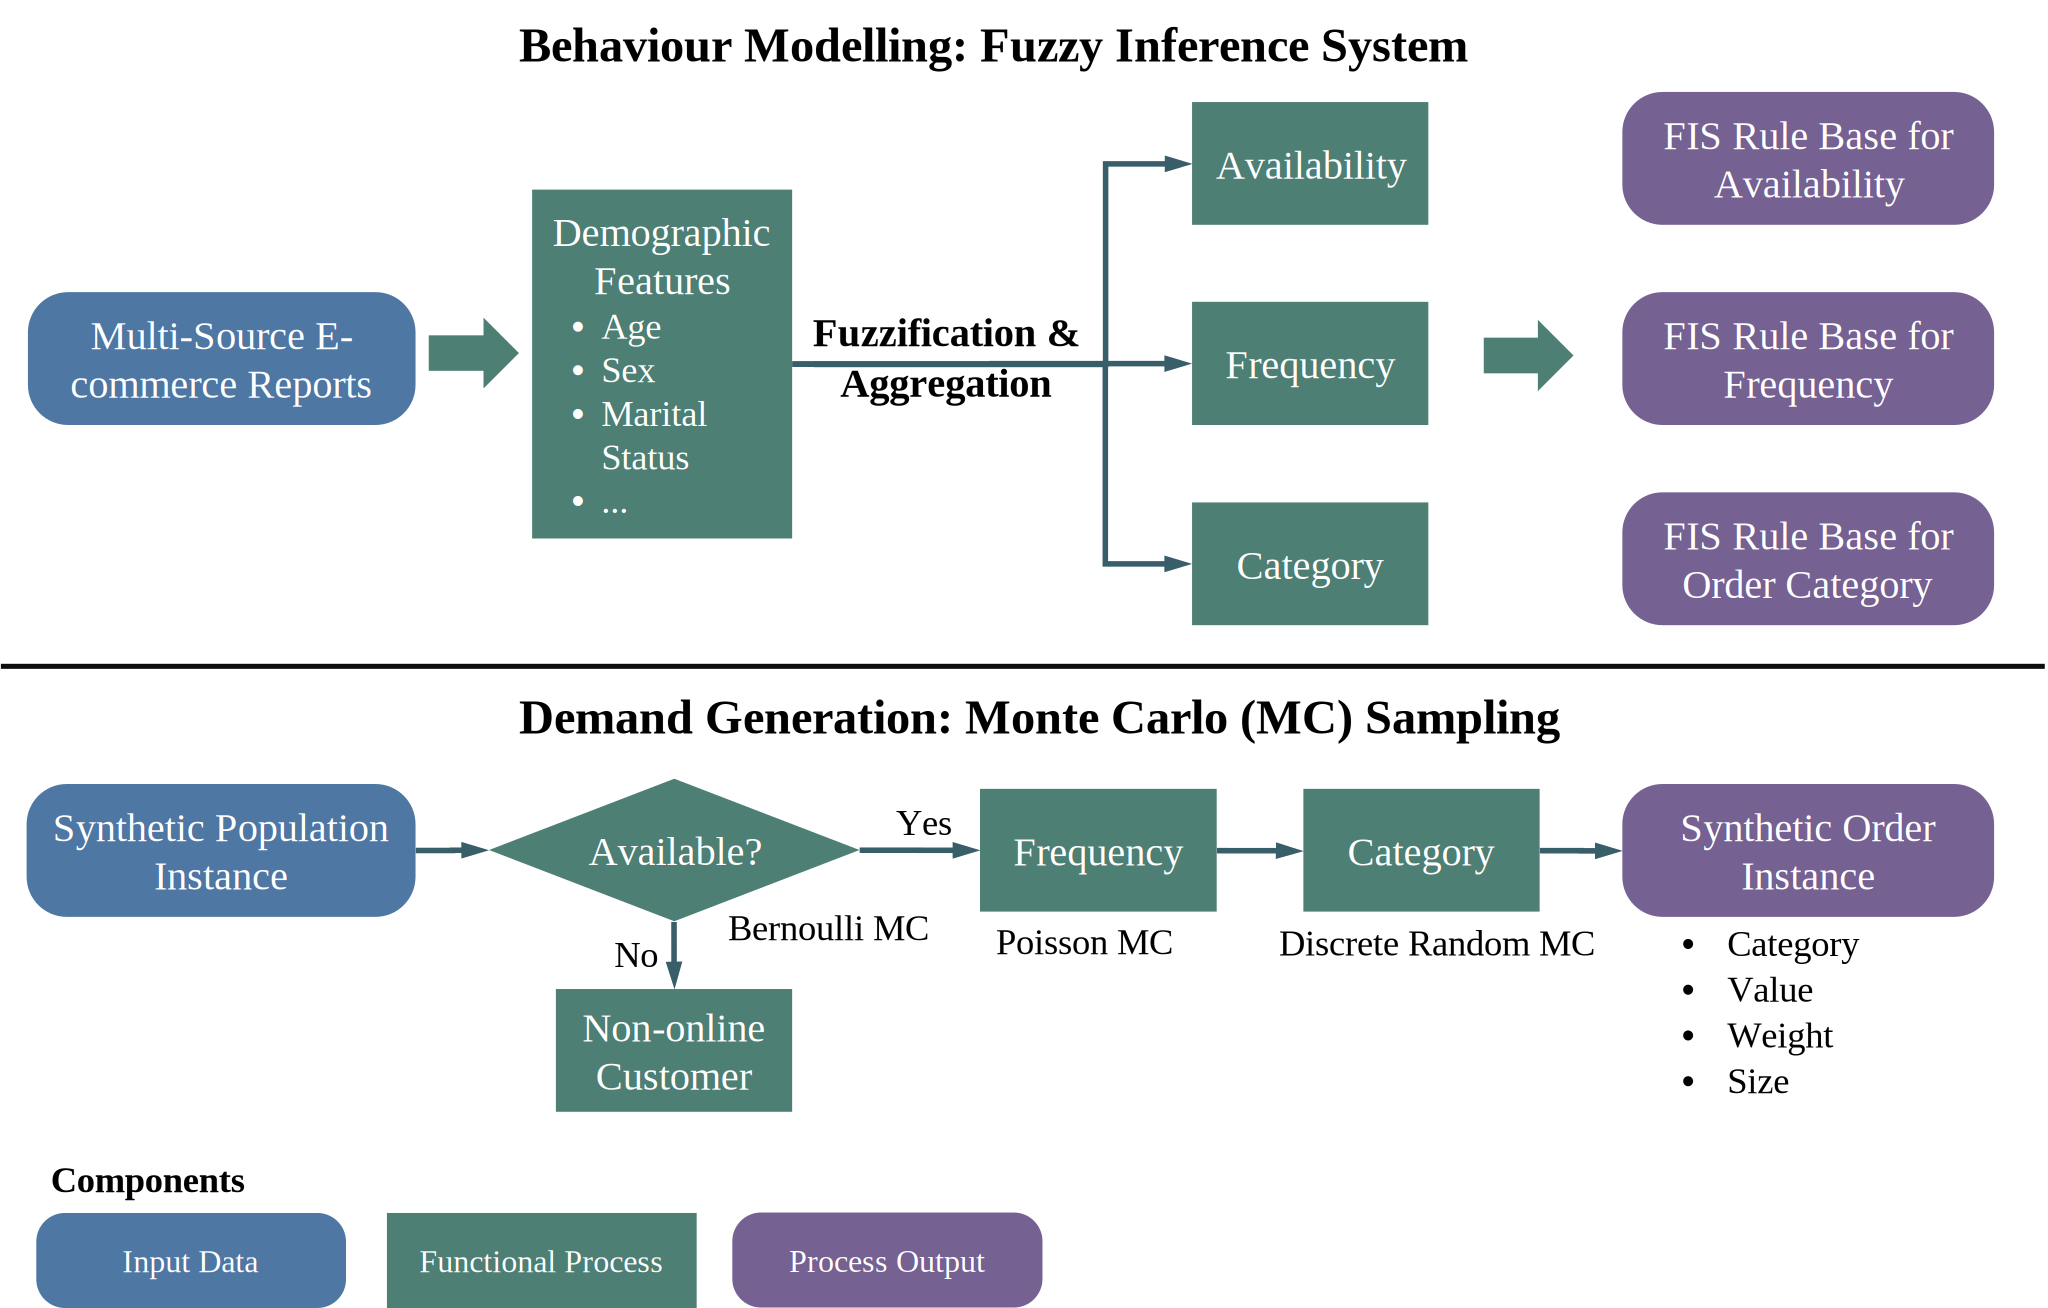
\includegraphics[width = 0.95\textwidth]{Figures/syn-order-flowchart.pdf}
  \caption{Synthetic Order Generation Flowchart}
  \label{fig:syn_ord_gen_frame}
\end{figure}

In this study, a multi-level FIS was developed to model consumer online shopping preferences in the UK. 
The system captures the relationships between demographic characteristics and purchasing behaviour across different product categories through a three-step modelling process.

First, feasibility perception was modelled to identify the potential online shopping population, or the customers.
Second, purchase frequency was incorporated to quantify how often consumers place orders within a given period. 
Third, product categories were considered to capture the diversity of products purchased by individuals.

By integrating these three steps, the multi-level FIS proposed a behavioural logic chain that enables a nuanced representation of consumer behaviour, linking demographic features, such as age, income, and employment, with both the frequency and variety of purchases. 
This approach allows the system to capture heterogeneity in consumer preferences and to provide more precise insights into purchasing patterns across diverse population segments.

\subsubsection{Fuzzy Logic Inference}

Unlike classical binary logic, fuzzy logic allows for partial truth values ranging between 0 and 1, enabling the system to capture the inherent uncertainty and vagueness of real-world phenomena.

\textit{Fuzzification} Each input variable is first mapped to a set of fuzzy linguistic variables through membership functions (MFs). 
Commonly used membership functions include triangular (Equation \ref{equ:MF_Tri}), trapezoidal (Equation \ref{equ:MF_Tra}), and Gaussian functions (Equation \ref{equ:MF_Gauss}). 

Triangular MF is defined by three parameters \(a\), \(b\), \(c\) (left, peak, right):

\begin{equation}
  \label{equ:MF_Tri}
  \mu_{\text{tri}}(x; a, b, c) =
  \begin{cases}
  0, & x \le a \\
  \frac{x-a}{b-a}, & a < x \le b \\
  \frac{c-x}{c-b}, & b < x \le c \\
  0, & x \ge c
  \end{cases}
\end{equation}

Trapezoidal MF is defined by four parameters \(a\), \(b\), \(c\) and \(d\) (left foot, left top, right top, right foot):

\begin{equation}
  \label{equ:MF_Tra}
  \mu_{\text{trap}}(x; a, b, c, d) =
  \begin{cases}
  0, & x \le a \\
  \frac{x-a}{b-a}, & a < x \le b \\
  1, & b < x \le c \\
  \frac{d-x}{d-c}, & c < x \le d \\
  0, & x \ge d
  \end{cases}
\end{equation}

Gaussian MF is defined by center \(c\) and standard deviation $\sigma$:

\begin{equation}
  \label{equ:MF_Gauss}
  \mu_{\text{gauss}}(x; c, \sigma) = \exp\left(-\frac{(x-c)^2}{2\sigma^2}\right)
\end{equation}

The degree of membership quantifies the extent to which an input belongs to a given fuzzy set, facilitating smooth transitions between linguistic categories.

Among the three commonly used MFs, the triangular membership function is simple, computationally efficient, and easy to interpret, making it particularly suitable for systems with limited computational resources. 
The trapezoidal membership function provides a plateau region, allowing a range of values to have full membership, which can offer slightly more flexibility in representing uncertain data. 
However, it introduces additional parameters, increasing model complexity. 
The Gaussian membership function produces smooth and continuous curves, which is beneficial for capturing gradual transitions in data; nevertheless, it requires more computational effort and careful tuning of the standard deviation parameter.

As indicated by Kosheleva \shortcite{Kosheleva2021}, in practical applications, triangular and trapezoidal MFs are the most efficient ones. 
Considering the trade-off between computational simplicity, interpretability, and modelling capability, the triangular membership function was selected for this study. 
The MFs of each input variable (antecedent), and output variable (consequent) are listed in Appendix \ref{tab:membership_fuc}.
Its straightforward definition and minimal parameters allow for efficient fuzzy inference while maintaining sufficient expressiveness to capture the relevant system dynamics.

\textit{Rule-Based Inference} The FIS applies a set of IF-THEN rules, which are either derived from expert knowledge or learned from data. 
For instance, a typical rule can be formulated as: 

\begin{itemize}
  \item IF input1 IS High AND input2 IS Medium THEN output IS High response
\end{itemize}

The rule evaluation is performed using fuzzy logic operators, where AND is typically modelled by the minimum operator and OR by the maximum operator.
In this study, we retained the default settings for these logic operators. 

\textit{Aggregation and Defuzzification} After evaluating all rules, the fuzzy outputs are aggregated into a single fuzzy set. 
To produce a crisp output, a defuzzification method is then applied. 
Depending on the application requirements, the FIS can be implemented as a Mamdani-type system, which produces fuzzy outputs and offers strong interpretability for control purposes, or a Sugeno-type system, which provides outputs as linear functions or constants and is suitable for optimisation and adaptive modelling. 
In this study, the centroid method is adopted within a Mamdani-type framework, owing to its widespread use and its ability to provide a balanced representation of the fuzzy output for control applications. 

This fuzzy logic approach allows the system to handle imprecise, noisy, or incomplete data and can model non-linear relationships without requiring explicit mathematical equations. 
It is particularly suitable for domains where human expertise or multiple fragmented information can be aggregated and codified into fuzzy rules. 

\subsubsection{Three-step E-commerce Customer Behaviour Chain Modelling} 

In this study, we proposed a three-stage fuzzy inference system to simulate the online shopping behaviour chain of individuals. 
The system proceeds through three sequential steps: availability (determining whether an individual is likely to engage in online shopping), frequency (estimating the number of online shopping orders within a given time period), and category (identifying the types of products the individual tends to purchase). 
This design aims to closely approximate real-world online shopping processes. 
The primary objective is to infer whether an individual has the potential to engage in online shopping, their likely shopping frequency, and the categories of products they are inclined to purchase. 

\textit{Availability} According to Eurostat \shortcite{eurostat_euro_statistics25}, around 77\% population place online orders. 
Therefore, the initial step is to use FIS to identify online customers from a synthetic population. And this is related to demographic features such as age and economic activity.

\textit{Frequency} To characterise individuals' shopping frequency within specific time intervals, we first categorised frequency levels as shown in the Table \ref{tab:freq_conversion} and extracted relevant information from data sources mentioned in Section \ref{sec:e-commerce_data}, which was then transformed into IF-THEN rules to fit the purchase frequency distributions across different person types. 

\begin{table}[htbp]
  \centering
  \caption{Order Frequency Table}
  \label{tab:freq_conversion}
  \begin{tabular}{c c c c c}
    \toprule
    \textbf{No.} & \textbf{Frequency} & \textbf{per Day} & \textbf{per Week} & \textbf{per Month} \\
    \midrule
    0 & Several times a day & 3.0000 & 21.0000 & 90.0000 \\
    1 & Daily & 1.0000 & 7.0000 & 30.0000 \\
    2 & 2-3 times a week & 0.3571 & 2.5000 & 10.7000 \\
    3 & Once a week & 0.1429 & 1.0000 & 4.3000 \\
    4 & 2-3 times a month & 0.0833 & 0.5814 & 2.5000 \\
    5 & Once a month & 0.0333 & 0.2326 & 1.0000 \\
    6 & Several times a year & 0.0137 & 0.0962 & 0.4200 \\
    7 & Less often & 0.0027 & 0.0192 & 0.0830 \\
    \bottomrule
  \end{tabular}
\end{table}

In the subsequent sampling process, these distributions are further transformed to obtain the expectation of order frequency within a given time window, using the frequency table \ref{tab:freq_conversion}, thereby enabling sampling that better reflects realistic consumption behaviour. 

\textit{Category} In the modelling of product categories, considering the requirements of downstream delivery scheme design and VRP-related optimisation problems, we not only distinguished between broad product categories but also incorporated critical factors such as volume, weight, and delivery time windows. 
On this basis, an appropriate generalisation of product classification was performed, as detailed in the Table \ref{tab:category_values}. 
Subsequently, we extracted IF-THEN fuzzy inference rules to model the purchase preferences of different person types for various product categories, thereby laying the foundation for subsequent delivery optimisation and strategy design.

\begin{table}[htbp]
  \centering
  \caption{Category Classification}
  \label{tab:category_values}
  \begin{tabularx}\textwidth{c X c X}
    \toprule
    \textbf{No.} & \textbf{Category Name} & \textbf{Size} & \textbf{Sub Category} \\
    \midrule
    0 & Lightweight Fashion \& Personal Care & Small & Clothing, Shoes, Accessories, Cosmetics, Body Care, Drugstore \& Health 
    \\
    1 & Small High-Value Electronics & Small & Consumer Electronics, Some Hobby Supplies 
    \\
    2 & Medium-Sized Consumer Goods & Medium & Food, Beverages, Household Care, Pet Products 
    \\
    3 & Cultural \& Entertainment Products & Small/Medium & Books/Music/Games, Sports, Toys \& Baby, Stationery \& Hobbies 
    \\
    4 & Medium-Sized Durable Home Goods & Medium & DIY \& Garden, Small Household Appliances 
    \\
    5 & Large Heavy Items & Large & Furniture, Large Household Appliances 
    \\
    6 & Travel \& Luggage Products & Medium & Luggage \& Bags \\
    \bottomrule
  \end{tabularx}
\end{table}

After the three-step modelling process, the availability-frequency-category process, we extracted a corresponding set of rules. 
For any individual or population with different demographic feature profiles, these rules can be used to calculate the probability distribution of outcomes at each decision step. 
These probability distributions provide the basis for subsequent Monte Carlo sampling.


\subsection{Synthetic Order Generation}
\label{sec:syn_ord_gen}

During the sampling stage, in order to reduce computation time, a representative-based calculation approach was adopted. 
Specifically, since large populations contain repeated individuals with identical demographic characteristics, we first extracted representative individuals, each corresponding to a group of people sharing the same e-commerce behavioural traits. 
In the multi-layer inference system, for the same group, the three-step decision probability distributions (availability, frequency, and category) are identical. 
Therefore, it is sufficient to compute the probability distributions for each representative and associate them with the entire synthetic population.

Availability refers to the probability that an individual may become an online customer, with a probability ranging from 0 to 1. 
Monte Carlo sampling is performed using a Bernoulli distribution (Equation \ref{equ:bernoulli}) based on this probability.

\begin{equation}
  \label{equ:bernoulli}
  \begin{aligned}
    X \sim \text{Bernoulli}(p)&, \\
    P(X=x) = p^x (1-p)^{1-x}&, \quad x \in \{0,1\}
    \end{aligned}
\end{equation}

Frequency refers to the number of orders one customer would place within the study period.
The number of orders is then assumed to follow a Poisson distribution (Equation \ref{equ:poisson}), which is typically used to model the number of discrete events occurring within a fixed period.
Therefore, the expectation of frequency is calculated using the order frequency table (Table \ref{tab:freq_conversion}), with each frequency category weighted by its corresponding probability. 
In this study, the time window is set to one week. 
Monte Carlo sampling is then applied based on these distributions.

\begin{equation}
  \label{equ:poisson}
  \begin{aligned}
    X \sim \text{Poisson}(\lambda)&, \\
    P(X = k) = \frac{\lambda^k e^{-\lambda}}{k!}&, \quad k = 0,1,2,\dots
    \end{aligned}
\end{equation}

Category refers to the type of products purchased, as listed in Table \ref{tab:category_values}. 
Monte Carlo sampling is conducted using random sampling from a discrete distribution (Equation \ref{equ:discrete}) to assign product categories for each order.

\begin{equation}
  \label{equ:discrete}
  \begin{aligned}
    X \sim \text{Discrete}(\{x_1, x_2, \dots, x_n\}&, \{p_1, p_2, \dots, p_n\}), \\
    P(X = x_i) = p_i&, \quad i = 1,2,\dots,n
    \end{aligned}
\end{equation}

Order details refer to order features such as order value, weight, and size. 
After obtaining the category of each order, these details were assigned accordingly.
Due to the insufficient statistical information (e.g., mean and variance) on the weight and size of different categories in last-mile delivery, we combined relevant sources \cite{statista_uk_shopping25_statistic} with the weight standards used when classifying the categories, assuming normal distributions for each category (Equation \ref{equ:normal}). 
Normal distribution sampling was then performed for the price and weight of each order. 

\begin{equation}
  \label{equ:normal}
  \begin{aligned}
    X \sim \mathcal{N}(\mu, \sigma^2)&, \\
    f_X(x) = \frac{1}{\sqrt{2 \pi \sigma^2}} \exp \Big( -\frac{(x-\mu)^2}{2\sigma^2} \Big)&, \quad x \in \mathbb{R}
  \end{aligned}
\end{equation}


This process in this subsection ultimately yields a set of synthetic order instances, each containing customer demographic attributes, address, and order details, including order category, value, and order weight. 
The resulting dataset provides a comprehensive basis for subsequent delivery optimisation and strategy design.


\subsection{Verification and Validation}
\subsubsection{Verification and Validation Framework}

In this study, we evaluated the proposed framework through both verification and validation. 
Verification evaluates the correctness of the framework itself, i.e., whether the framework's logic and methodology conform to the design specifications.
Validation, on the other hand, assesses whether the proposed framework achieves the intended objectives, that is, whether the generated results resemble the real-world data. 
Since our focus is on statistically and aggregately validating the synthetic data, we employed an indicator that measures the similarity of different distributions, specifically, the Jensen-Shannon Divergence (JSD) for quantitative assessment. 

Based on the proposed population-order two-step framework, the verification and validation process is conducted on two levels.
First, verification is evaluated as the simulation scale increases. We examine whether the marginal distributions of the synthetic data (population, orders) converge toward those of the real-world data. 
The assessment of asymptotic consistency demonstrates the correctness of the synthetic instances.
Second, validation is evaluated once the asymptotic results reach convergence.
Smaller differences between the synthetic instances and real-world data, ideally below a practical threshold, indicate higher fidelity and validate the effectiveness of the framework.


\subsubsection{Measure of Distribution Similarity, Jensen-Shannon Divergence}

Since our focus is on statistically and aggregately validating the synthetic data, we compared several measures to quantify the similarity between distributions. 
These include the Kullback-Leibler Divergence (KLD) \cite{measure_KLD1951}, Kolmogorov-Smirnov (KS) Statistic \cite{measure_KSStatistic1951},  Cosine Similarity \cite{measure_Cosine1975}, Total Variation Distance (TVD) \cite{measure_TVDistance1960} and Jensen-Shannon Divergence (JSD) \cite{measure_JSD1991}.

The KLD measures the information loss or discrepancy between two probability distributions, but it is asymmetric and is sensitive to zero probability. 
The KS Statistic quantifies the maximum difference between two cumulative distribution functions.
Cosine Similarity takes the two distributions as vectors and measures the directional similarity between these two vectors.
The TVD indicator quantifies the maximum absolute difference between two probability distributions.
The JSD is a symmetric version of KLD that measures divergence relative to the average distribution 
By mapping both distributions to a midpoint and evaluating the information divergence from it, JSD provides a bounded and symmetric measure.
It is numerically stable and widely applied for high-dimensional probability distribution comparisons and generative modelling.
Therefore, in this study, we adopted JSD as the primary indicator for the verification and validation process.

Given two probability distributions \(P\) and \(Q\), the JSD is defined as:

\begin{equation}
  \label{equ:JSDdefin}
  \begin{aligned}
    JSD(P||Q) &= \sqrt{\frac{1}{2}D_{KL}(P||M) + \frac{1}{2}D_{KL}(Q||M) }\\
    D_{KL}(P||Q) &= \sum_i P(i) \log \frac{P(i)}{Q(i)}\\
    M &= \frac{1}{2}(P+Q)
  \end{aligned}
\end{equation}

where \(M\) is the midpoint distribution and \(D_{KL}\) is the Kullback-Leibler Divergence.

The JSD ranges from 0 (identical distributions) to 1 (completely dissimilar). 
Smaller JSD values correspond to smaller differences between distributions \(P\) and \(Q\).


\subsubsection{Synthetic Population Validation}

In the population validation process, since the synthetic population is generated at the LSOA level, we performed cross-validation using marginal statistics at a higher-level administrative unit, namely the LAD, to ensure that the marginal distributions of different demographic attributes in the synthetic data align with those of the real population. 

Specifically, the populations of all LSOAs within each LAD were aggregated, and the resulting distributions were compared against the actual population distributions reported in the census statistics. 
When calculating the JSD, we first obtained the JSD value for each individual LAD. 
In total, 14 LADs in Inner London were evaluated, each producing a JSD value. 
The final validation result for the ILA was then defined as the average JSD across these 14 LADs.
Considering the priority sampling approach described in Section \ref{sec:samplePop}, which favours high-proportion population groups, the generated population for a given population size is deterministic rather than stochastic.
Therefore, validation was conducted across a range of synthetic population sizes, and JSD was computed to examine whether it decreases as the population scale increases, thereby demonstrating the asymptotic consistency of the synthetic population.


\subsubsection{Synthetic Order Validation}
\label{sec:method_order_val}

For order validation, two aspects were considered. 
First, the synthetic orders themselves were validated by comparing their category distributions with those of actual order data. 
By comparing the category distributions of synthetic orders with those of the real UK online orders \cite{statista_uk_shopping25_statistic}, the realism and plausibility of the synthetic orders were quantitatively assessed.
Second, customer-based validation was performed to assess whether the attribute distributions (e.g., age) of potential online customers, identified through the FIS framework, match those of real-world UK online customers \cite{statista_uk_shopping25_statistic}. 
To ensure objectivity, independent third-party data was employed, ensuring the data used for validation is independent from the data used in the model fitting process. 

Since the generation of synthetic orders depends only on customer characteristics rather than spatial locations, we selected the ILA synthetic population with the highest data accuracy as the basis for order simulation. 
Specifically, orders were generated by sampling different proportions of individuals from this synthetic population.

During the sampling process, the order generation involves Monte Carlo sampling based on specified distributions and their probabilities, which inevitably introduces randomness. 
To avoid evaluation results being biased by the stochastic nature of a single random process, we employed multiple random seeds to repeatedly conduct sampling and order generation under the same population size. 
For each run, the JSD was computed, thereby ensuring more robust and reliable evaluation results.


\section{Case Study and Results}
\label{sec:results}

\subsection{Research Area}
This project is focused on the Inner London Area (ILA), a term often used in statistics and planning, including 14 boroughs in the London Plan \shortcite{london2021plan}. Different from the area in Central London and the Greater London Area (GLA), it is a core group of boroughs that form the central part of the capital.
The comparison of ILA and GLA is shown in Figure \ref{fig:london_map}.

\begin{figure}[htbp]
  \centering
  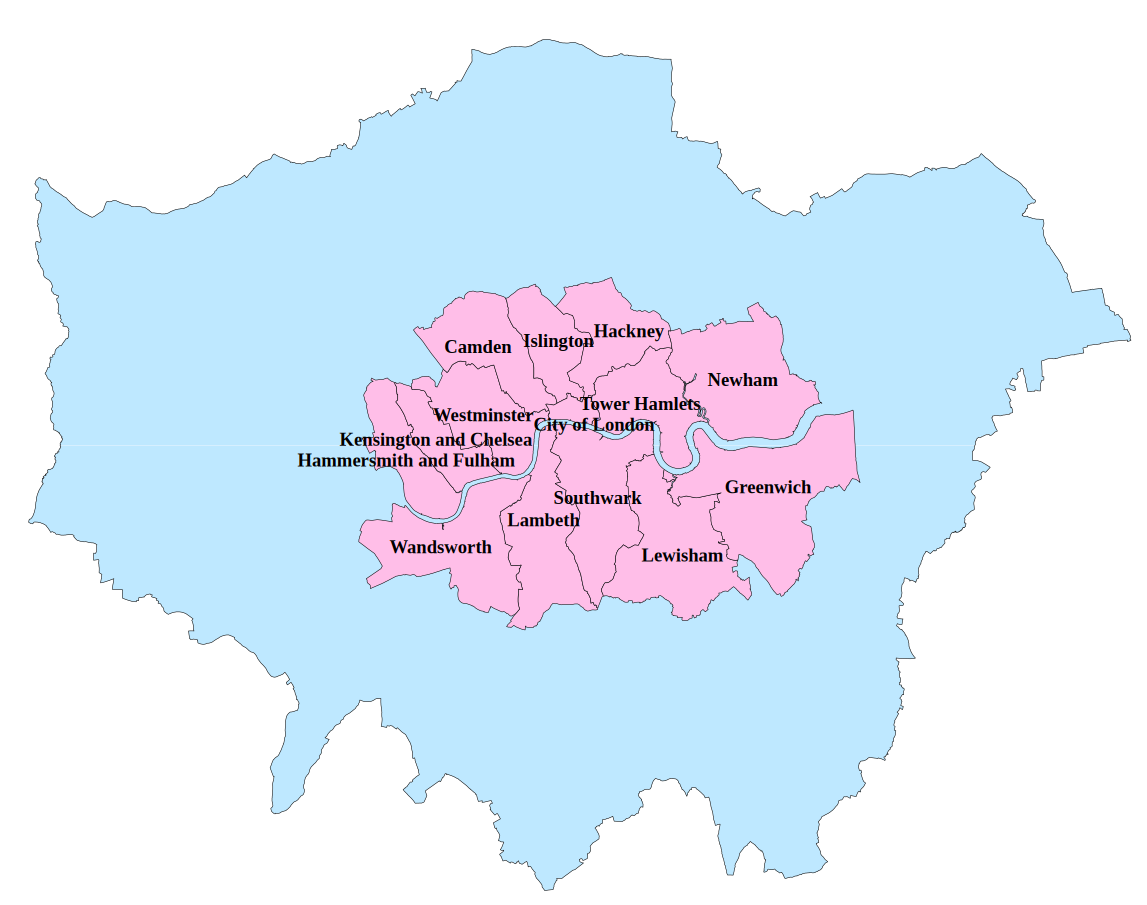
\includegraphics[width=0.8\textwidth]{Figures/london_map.pdf}
  \caption{Inner London Area and Greater London Area}
  \label{fig:london_map}
\end{figure}

\subsection{Synthetic Population}

We employed the IPF method for various population scales, with the relevant algorithm parameters and experimental parameters listed in the Table \ref{tab:simu_par_pop}. 

\begin{table}[htbp]
  \centering
  \caption{Algorithm and Experimental Parameters}
  \label{tab:simu_par_pop}
  \begin{tabularx}{0.9\textwidth}{l X X}
    \toprule
    \textbf{Type} & \textbf{Name} & \textbf{Value} \\
    \midrule
    IPF Parameter & Max Iteration & 1,000 \\
    IPF Parameter & Stop Threshold & 0.001 \\
    Experimental Parameter & Population Size & 10 values for each magnitude ($10^3 - 2 \times 10^6$) \\
    Experimental Parameter & Output Format & csv, gpkg, shp files\\
    \bottomrule
  \end{tabularx}
\end{table}

The final synthetic population data is presented in the form of a dataframe in different file formats, encompassing all population feature variables, with the example data shown in the Table \ref{tab:synpop_sample}.

\begin{table}[htbp]
  \centering
  \caption{Synthetic Population Data Sample ($2\times10^6$)}
  \label{tab:synpop_sample}
  \begin{tabular}{l c c c c c}
    \toprule
    \textbf{Person ID} & \textbf{Age} & \textbf{Sex} & \textbf{\makecell{Economic \\ Activity}} & $\mathbf{\cdots}$ & \textbf{Location*} \\
    \midrule
    ID\_00000000 & 0 & 0 & 0 & $\cdots$ & POINT (526470.3633 183249.8411) \\
    ID\_00000001 & 0 & 0 & 0 & $\cdots$ & POINT (526442.3315 183184.6906) \\
    ID\_00000002 & 0 & 0 & 0 & $\cdots$ & POINT (526368.7540 183190.1211) \\
    $\vdots$ & $\vdots$ & $\vdots$ & $\vdots$ & $\cdots$ & $\vdots$ \\
    ID\_01999998 & 3 & 1 & 0 & $\cdots$ & POINT (522008.0873 172633.4987) \\
    ID\_01999999 & 3 & 1 & 0 & $\cdots$ & POINT (522375.9823 173094.8757) \\
    \bottomrule
  \end{tabular}
  \vspace{1mm} \par
  \textit{*Note: Coordinates are expressed in the EPSG:27700 coordinate system, consistent with the commonly used coordinate reference system in the UK.}
\end{table}

The JSD curves computed for different population sizes are presented in the Figure \ref{fig:jsd-pop}.
Figure \ref{fig:jsd-pop} shows the change in JSD for various population attributes across different synthetic population sizes. 
Overall, as the synthetic population size increases, the JSD for nearly all attributes decreases. 
This indicates that with larger sizes, the generated population distribution across each feature becomes closer to the real-world population, reflecting improved simulation accuracy of the model.

\begin{figure}
  \centering
  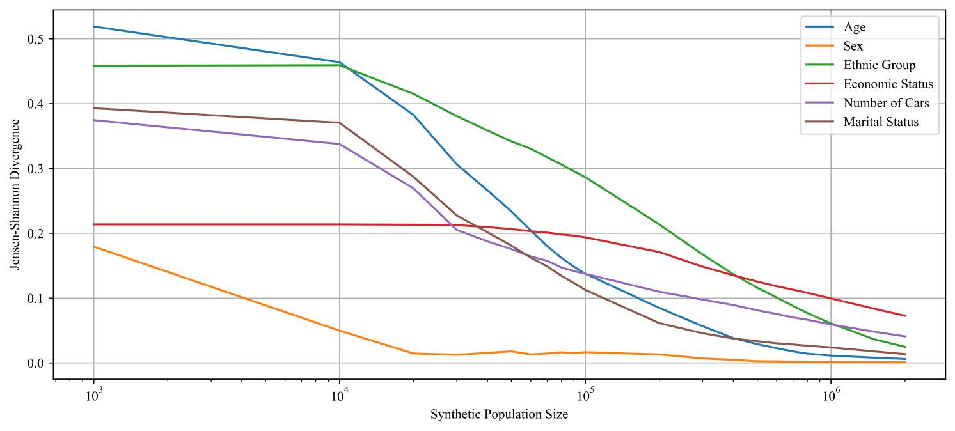
\includegraphics[width=0.95\textwidth]{Figures/jsd-pop.pdf}
  \caption{Jensen-Shannon Divergence by Demographic Features}
  \label{fig:jsd-pop}
\end{figure}

For specific attributes, gender has the lowest JSD and drops quickly even at smaller population sizes, suggesting that the gender distribution is easy to simulate accurately. 
Age and ethnic group start with relatively high JSD values but decrease significantly as population size increases, especially between $10^4$ and $10^5$. 
Economic status shows minimal change, with JSD starting relatively low and decreasing only slightly, indicating that its distribution is either easier to simulate or inherently less variable. 
The number of cars and marital status initially have higher JSD values but gradually decrease as the population grows, stabilising once the population reaches above $10^5$.

At small population sizes ($10^3$ to $10^4$), JSD for age, ethnicity, marital status, and number of cars is relatively high, showing that these attributes are harder to simulate accurately with limited samples. 
When the population exceeds $10^5$, JSD for most attributes approaches below 0.05, indicating that the generated distributions nearly match the real distributions and that increasing population size leads to progressively consistent simulation results.

In conclusion, as the population size increases, the differences between generated and real distributions shrink across all attributes, showing that the synthetic method performs robustly with large samples, achieving verification. 
Furthermore, the asymptotic values are all below 0.1, with most feature values falling below 0.05, further confirming the effectiveness of the IPF method in generating synthetic populations and demonstrating successful validation.


\subsection{Synthetic Order}

In the e-commerce modelling process, we extracted and integrated the IF-THEN rules for each step of the FIS from the data sources mentioned in Table \ref{tab:uk_ecommerce_sources}. 
The complete set of MFs for each variable is listed in Appendix Table \ref{tab:membership_fuc}. 
Part of the rules are listed in the Table \ref{tab:rlue_base_avail}, \ref{tab:rlue_base_freq}, \ref{tab:rlue_base_cate}. 
The complete rules can be found in Appendix \ref{tab:rlue_base_avail_all}, \ref{tab:rlue_base_freq_all}, and \ref{tab:rlue_base_cate_all}, respectively.

\begin{table}[htbp]
  \centering
  \caption{IF-THEN Rule Base for Availability (Partial)}
  \label{tab:rlue_base_avail}
  \begin{tabularx}{0.9\textwidth}{c X}
    \toprule
    \textbf{No.} & \textbf{Rule} \\
    \midrule
    1 & IF age[\textit{young\_adult}] OR age[\textit{adult}] THEN response[\textit{high}] \\
    2 & IF economic\_activity[\textit{employed}] OR economic\_activity[\textit{unemployed}] THEN response[\textit{medium}] \\
    3 & IF age[\textit{senior}] AND economic\_activity[\textit{inactive}] THEN response[\textit{low}] \\
    \bottomrule
  \end{tabularx}
\end{table}

\begin{table}[htbp]
  \centering
  \caption{IF-THEN Rule Base for Frequency (Partial)}
  \label{tab:rlue_base_freq}
  \begin{tabularx}{0.9\textwidth}{c c X}
    \toprule
    \textbf{Type} & \textbf{No.} & \textbf{Rule} \\
    \midrule
    Multi Daily & 1 & IF age[\textit{young\_adult}] THEN response[\textit{low}] \\
    Multi Daily & 2 & IF age[\textit{senior}] THEN response[\textit{low}] \\
    Weekly 2-3 Times & 1 & IF age[\textit{young\_adult}] THEN response[\textit{medium}] \\
    Weekly 2-3 Times & 2 & IF age[\textit{adult}] THEN response[\textit{high}] \\
    \bottomrule
  \end{tabularx}
\end{table}

\begin{table}[htbp]
  \centering
  \caption{IF-THEN Rule Base for Order Category (Partial)}
  \label{tab:rlue_base_cate}
  \begin{tabularx}{0.9\textwidth}{c c X}
    \toprule
    \textbf{Type} & \textbf{No.} & \textbf{Rule} \\
    \midrule
    Cloth \& Personal Care & 1 & IF age[\textit{young\_adult}] AND sex[\textit{female}] THEN response[\textit{high}] \\
    Cloth \& Personal Care & 2 & IF age[\textit{adult}] AND sex[\textit{female}] THEN response[\textit{high}] \\
    High-Value Electronics & 1 & IF age[\textit{young\_adult}] AND sex[\textit{female}] THEN response[\textit{low}] \\
    High-Value Electronics & 2 & IF age[\textit{adult}] AND sex[\textit{female}] THEN response[\textit{medium}] \\

    \bottomrule
  \end{tabularx}
\end{table}

After modelling the e-commerce behaviour, we used the FIS to generate synthetic orders based on synthetic population.
We sampled different percentages of the population from the population with the highest simulation accuracy, specifically, $2\times10^6$, and applied the proposed multi-level FIS.
Algorithm and experimental parameters are shown in Table \ref{tab:simu_par_ord}. 


\begin{table}[htbp]
  \centering
  \caption{Algorithm and Experimental Parameters}
  \label{tab:simu_par_ord}
  \begin{tabularx}{0.9\textwidth}{c X X}
    \toprule
    \textbf{Type} & \textbf{Name} & \textbf{Value} \\
    \midrule
    FIS Parameter & Membership Function & Triangular \\
    FIS Parameter & AND Aggregation Function & fmin \\
    FIS Parameter & OR Aggregation Function & fmax \\
    FIS Parameter & Defuzzification Function & Centroid \\
    Experimental Parameter & Population Size & 10 values for each magnitude ($10^3 - 2 \times 10^6$) \\
    Experimental Parameter & Random Seed & 0, 1, 2, \dots,19, 42 \\
    \bottomrule
  \end{tabularx}
\end{table}

We first validated the categories of the orders. 
We incorporated an independent third-party data source \cite{statista_uk_shopping25_statistic} to obtain the distribution of actual online shopping orders in UK. 
This distribution was then compared with the synthetic orders generated under different population scales and random seeds. 
The JSD between the two distributions was computed to assess the fidelity of the synthetic orders, as shown in the Figure \ref{fig:jsd_order}.

\begin{figure}[htbp]
  \centering
  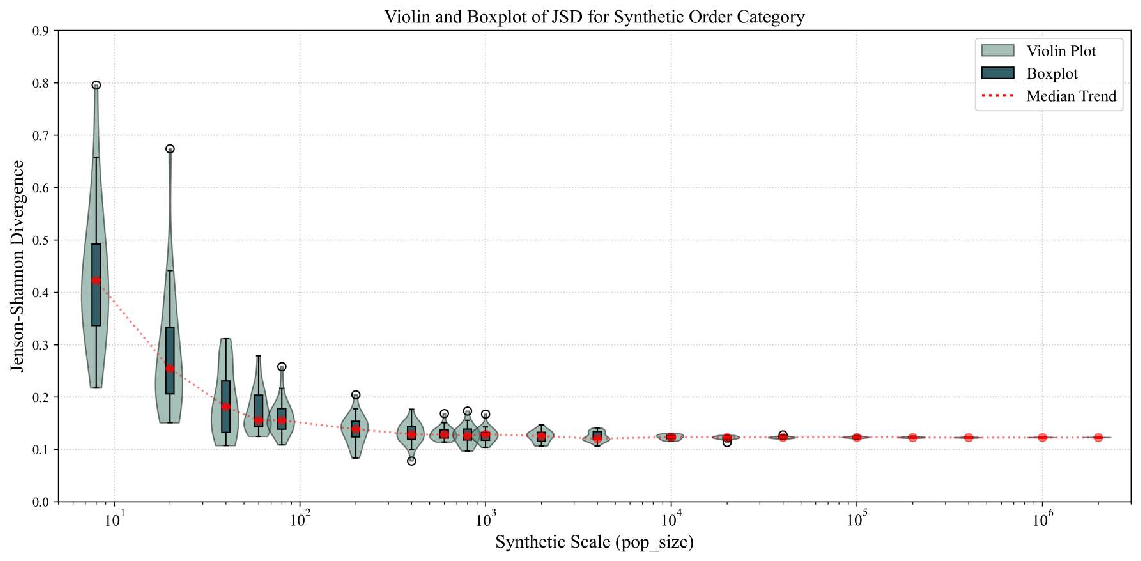
\includegraphics[width=0.95\textwidth]{Figures/jsd-ord.pdf}
  \caption{Jenson-Shannon Divergence of Synthetic Order Category}
  \label{fig:jsd_order}
\end{figure}

As shown in Figure \ref{fig:jsd_order}, the JSD decreases monotonically with increasing population size, with a particularly rapid decline below 100, indicating that the synthetic orders generated by the FIS framework quickly converge toward the true distribution. 
Multiple repetitions with different random seeds reveal that, for small sample sizes, especially below 100, the results fluctuate significantly and the synthetic outcomes are unstable. 
As the simulation scale increases, the JSD gradually stabilises, and for population sizes above 1,000, it remains at a low level (approximately 0.12), demonstrating that larger samples better approximate the true distribution.

Overall, the accuracy of the synthetic instances is closely related to the simulation scale, with larger populations yielding higher-quality synthetic data. 
The rapid convergence of JSD and its low final value further confirms the effectiveness of the model's verification and validation. 
As the population size continues to grow, the JSD reaches a plateau around 0.12, suggesting that the error transitions from being dominated by variance due to small sample size to being dominated by structural errors in the FIS framework or data.

The stability threshold indicates that, to achieve instances that fit the real-world order distribution, the synthetic population size should at least be larger than 100, beyond which variance is effectively controlled. 

Similarly, we examined the demographic feature distribution of consumers. 
Since some report indicates that not all individuals choose to engage in online shopping \cite{eurostat_euro_statistics25}, it is necessary to validate the demographic distribution specifically for the actual online shopping population. 
We summarised the customer attribute statistics under different population scales and random seeds and compared the customer profiles with the reference data from \textit{UK Online Shopping Behavior Report} \cite{statista_uk_shopping25_statistic}.
The results are shown in Figure \ref{fig:jsd-age}.

\begin{figure}[htbp]
  \centering
  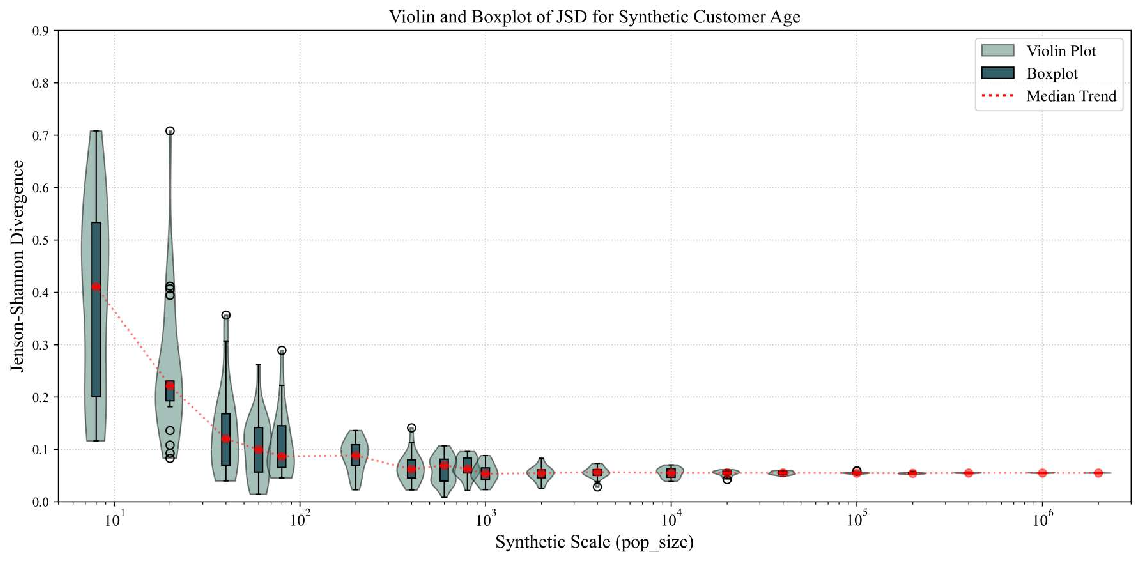
\includegraphics[width=0.95\textwidth]{Figures/jsd-age.pdf}
  \caption{Jenson-Shannon Divergence of Customer Age}
  \label{fig:jsd-age}
\end{figure}

Figure \ref{fig:jsd-age} shows that as the synthetic population size increases, the JSD values exhibit a general decline and gradually converge, indicating that larger samples provide a closer approximation to the real-world customer profile.

At smaller scales, the JSD values are more dispersed, with some reaching as high as around 0.7. 
This suggests that when the synthetic population size is insufficient, the generated distributions tend to be unstable and deviate considerably from the actual distribution.
With increasing scale, the JSD values decrease substantially and become more concentrated. 
Most results converge within the range of 0.025-0.075, suggesting that the discrepancies between the synthetic and real distributions are significantly reduced. 
At larger scales, the JSD values stabilise around 0.05 with minimal fluctuations, indicating that further increases in population size yield limited improvements in fidelity. 

The results demonstrate that as the synthetic population size increases, the generated customer age distribution progressively approaches the real-world distribution, thereby validating the effectiveness of the proposed FIS method in this demographic dimension.
When the population size reaches 1,000 or above, the JSD values consistently remain below 0.1, suggesting sufficient accuracy of the synthetic orders. 
Accordingly, for downstream applications aiming to approximate real-world last-mile scenarios, a synthetic population size exceeding 1,000 is recommended.

In summary, based on the validation of both order categories and consumer demographic characteristics, the results collectively confirm the effectiveness of the proposed FIS framework. 
As indicated by the JSD results shown in Figure \ref{fig:jsd_order} and Figure \ref{fig:jsd-age}, a population size greater than 1,000 is recommended in practical applications to ensure sufficient similarity to the real-world scenarios in downstream simulation.


\subsection{Web-based Result Visualisation}

After generating the synthetic population and order instance, a web-based visualisation method was adopted to present the results. 
To address the issue of point over-density on the webpage, a sampling strategy was applied, and it is user-defined, ensuring that the displayed data remains both representative and visually interpretable.
The visualisation on the webpage for the synthetic population and the synthetic orders are demonstrated as Figure \ref{fig:map_synpop} and Figure \ref{fig:map_synord}.

\begin{figure}
  \centering
  \includegraphics[width=0.95\textwidth]{Figures/synpop-map.pdf}
  \caption{Web-based Visualisation of Synthetic Population}
  \label{fig:map_synpop}
\end{figure}

\begin{figure}
  \centering
  \includegraphics[width=0.95\textwidth]{Figures/synord-map.pdf}
  \caption{Web-based Visualisation of Synthetic Order}
  \label{fig:map_synord}
\end{figure}


\section{Conclusion and Discussion}
\label{sec:conclusion}

This study addresses the data privacy challenges in last-mile delivery orders and the limitations of existing order demand data, which often neglect consumer purchase preferences and demographic characteristics. 
We propose a population-feature-based method for generating synthetic orders, consisting of two main steps. 
First, a synthetic population of the ILA are generated using census data. 
Second, a FIS is constructed to model online purchase preferences based on demographic features, following a three-stage online shopping logic chain: online availability, purchase frequency, and product category. 
By integrating this FIS with the MC sampling framework, synthetic orders are generated that align with real-world population preferences.

Cross-validation with independent third-party data demonstrates that the proposed method effectively captures actual consumer purchase behaviour, confirming its validity in modelling both order generation and demographic-based purchase preferences. 
Validation results also indicate that, in subsequent logistics simulations, if the goal is to obtain order volumes that better reflect market behaviour, it is advisable to set the number of generated synthetic order instances to larger than 100. 
This scale ensures that the generated orders are consistent with the shopping preferences of the ILA population.

This study exhibits strong extensibility. 
Methodologically, it proposes an open-source, reproducible scenario generation pipeline tailored to ILA, capable of producing synthetic order instances at specified scales on demand. 
At the model level, it incorporates consumer demographic characteristics and is supported by an extensible rule base, making it easy to transfer and expand.
  other purchase preferences, enabling the simulation of more diverse and realistic scenarios.

In the future, this framework can incorporate additional data sources and delivery preferences, such as delivery time windows, delivery modes, and delivery locations (e.g., self-pickup or parcel lockers), can be further incorporated. 
By calibrating these choices with data from industry reports, the framework can produce more fine-grained and realistic order-simulation instances, supporting downstream last-mile logistics simulations and generating synthetic orders at varying scales to accommodate different scenarios. 


\section*{Acknowledgement}

Time has flown by in the blink of an eye, and before I realised it, my master's journey has come to an end. 
From spring to autumn, I have finally reached the completion of my dissertation. 
Here, I would like to express my heartfelt gratitude to all those who have supported and helped me along the way.

First and foremost, I would like to express my deepest gratitude to my supervisor, Professor Angeloudis. 
His passion for academic research and teaching has deeply inspired me and strengthened my determination to choose him as my dissertation advisor. 
His profound insights into logistics, as well as his invaluable guidance throughout this process, have provided me with tremendous inspiration and support.

I am also sincerely grateful to Keyang, our doctoral mentor. 
His rigorous academic attitude has always been a model for me. 
Whenever I encountered setbacks or confusion, he encouraged me with patience, pointed out deficiencies in my ideas, content, and direction, and helped me to continuously improve and refine my research. 
His support has been of great significance to the successful completion of my dissertation. 
I sincerely wish him every success in his future endeavours.

I would also like to thank the friends I met during my MSc studies. Conversations with you not only helped me relieve pressure during stressful times but also often sparked new ideas for my project. 
In particular, I would like to thank Luis, Thomas, and Sami for your companionship and support, which have given me precious friendship on this academic journey. 
I wish you all the very best in the future.

Finally, I owe my deepest gratitude to my family. 
In those late nights of writing and struggling with ideas, it was your understanding, encouragement, and love that kept me going. 
Without your support, I would not have been able to achieve what I have today.

\bibliographystyle{authordate2}
\bibliography{refs}

\newpage
\appendix
\section{List of Abbreviation}

\DTLsort{abbr}{acronyms}

% Abbreviation Table
\begin{center}
  \begin{tabular}{l l}
    \textbf{Abbreviation} & \textbf{Full Form} \\
    \midrule
    \DTLforeach{acronyms}{\abbr=abbr,\full=full}{%
      \abbr & \full \\%
    }
  \end{tabular}
\end{center}

\newpage

\section{Fuzzy Inference System}
\label{apdx:fis_rules}

% Membership functions
\begin{longtable}[c]{l}
  \caption{Membership Function for Antecedent and Consequent
  \label{tab:membership_fuc}}\\

  \endfirsthead
 
  \multicolumn{1}{l}{\textit{Continuation of Table \ref{tab:membership_fuc}}}\\
  \endhead
  
  \midrule
  \multicolumn{1}{r}{\textit{Continued on next page}} \\
  \endfoot
 
  \bottomrule
  \endlastfoot

  \toprule
  \multicolumn{1}{c}{\textbf{Input Variables (Antecedents)}} \\
  \midrule

  \multicolumn{1}{l}{\textbf{Age}: 0 = 0--15, 1 = 16--29, 2 = 30--49, 3 = 50+} \\[0.1em]
  age[\textit{child}] = fuzz.trimf(age.universe, [0, 0, 1]) \\
  age[\textit{young\_adult}] = fuzz.trimf(age.universe, [0, 1, 2]) \\
  age[\textit{adult}] = fuzz.trimf(age.universe, [1, 2, 3]) \\
  age[\textit{senior}] = fuzz.trimf(age.universe, [2, 3, 3]) \\
  \midrule

  \multicolumn{1}{l}{\textbf{Sex}: 0 = Female, 1 = Male} \\[0.2em]
  sex[\textit{female}] = fuzz.trimf(sex.universe, [0, 0, 1]) \\
  sex[\textit{male}] = fuzz.trimf(sex.universe, [0, 1, 1]) \\
  \midrule

  \multicolumn{1}{l}{\textbf{Marital Status}: 0 = Single, 1 = Married, 2 = Divorced/Widowed} \\[0.1em]
  marital\_status[\textit{single}] = fuzz.trimf(marital\_status.universe, [0, 0, 1]) \\
  marital\_status[\textit{married}] = fuzz.trimf(marital\_status.universe, [0, 1, 2]) \\
  marital\_status[\textit{divorced\_widowed}] = fuzz.trimf(marital\_status.universe, [1, 2, 2]) \\
  \midrule

  \multicolumn{1}{l}{\textbf{Economic Activity}: 0 = Employed, 1 = Unemployed, 2 = Inactive} \\[0.1em]
  eco\_act[\textit{employed}] = fuzz.trimf(eco\_act.universe, [0, 0, 1]) \\
  eco\_act[\textit{unemployed}] = fuzz.trimf(eco\_act.universe, [0, 1, 2]) \\
  eco\_act[\textit{inactive}] = fuzz.trimf(eco\_act.universe, [1, 2, 2]) \\
  \midrule

  \multicolumn{1}{l}{\textbf{Ethnic Group}: 0 = Asian, 1 = Black, 2 = Mixed, 3 = White, 4 = Other} \\[0.1em]
  ethnic[\textit{asian}] = fuzz.trimf(ethnic.universe, [0, 0, 1]) \\
  ethnic[\textit{black}] = fuzz.trimf(ethnic.universe, [0, 1, 2]) \\
  ethnic[\textit{mixed}] = fuzz.trimf(ethnic.universe, [1, 2, 3]) \\
  ethnic[\textit{white}] = fuzz.trimf(ethnic.universe, [2, 3, 4]) \\
  ethnic[\textit{other}] = fuzz.trimf(ethnic.universe, [3, 4, 4]) \\
  \midrule

  \multicolumn{1}{l}{\textbf{Number of Cars/Vans}: 0 = None, 1 = One, 2 = Two, 3 = Three or More} \\[0.1em]
  cars[\textit{none}] = fuzz.trimf(cars.universe, [0, 0, 1]) \\
  cars[\textit{one}] = fuzz.trimf(cars.universe, [0, 1, 2]) \\
  cars[\textit{two}] = fuzz.trimf(cars.universe, [1, 2, 3]) \\
  cars[\textit{three\_or\_more}] = fuzz.trimf(cars.universe, [2, 3, 3]) \\ [0.1em]

  \toprule
  \multicolumn{1}{c}{\textbf{Output Variable (Consequent)}} \\
  \midrule

  \multicolumn{1}{l}{\textbf{Response Probability}: 0--100} \\[0.1em]
  response[\textit{low}] = fuzz.trimf(response.universe, [0, 0, 40]) \\
  response[\textit{medium}] = fuzz.trimf(response.universe, [30, 50, 70]) \\
  response[\textit{high}] = fuzz.trimf(response.universe, [60, 100, 100]) \\

\end{longtable}
  
% IF-THEN Rule Base for Availability
\begin{table}[htbp]
  \centering
  \caption{IF-THEN Rule Base for Availability}
  \label{tab:rlue_base_avail_all}
  \begin{tabularx}{0.9\textwidth}{c X}
    \toprule
    \textbf{No.} & \textbf{Rule} \\
    \midrule
    1 & IF age[\textit{young\_adult}] OR age[\textit{adult}] THEN response[\textit{high}] \\
    2 & IF economic\_activity[\textit{employed}] OR economic\_activity[\textit{unemployed}] THEN response[\textit{medium}] \\
    3 & IF age[\textit{senior}] AND economic\_activity[\textit{inactive}] THEN response[\textit{low}] \\
    4 & IF age[\textit{young\_adult}] AND economic\_activity[\textit{employed}] THEN response[\textit{high}] \\
    \bottomrule
  \end{tabularx}
\end{table}

% IF-THEN Rule Base for Frequency
\begin{longtable}[c]{c c l}
  \caption{IF-THEN Rule Base for Frequency 
  \label{tab:rlue_base_freq_all}}\\
  \toprule
  \textbf{No.} & \textbf{Frequency} & \textbf{Rule} \\
  \midrule
  \endfirsthead
 
  \multicolumn{3}{l}{\textit{Continuation of Table \ref{tab:rlue_base_freq_all}}}\\
  \toprule
  \textbf{No.} & \textbf{Frequency} & \textbf{Rule} \\
  \midrule
  \endhead
 
  \midrule
  \multicolumn{3}{r}{\textit{Continued on next page}} \\
  \endfoot
 
  \bottomrule
  \endlastfoot
 
  1 & Several times a day & IF age[\textit{young\_adult}] THEN response[\textit{low}] \\
  2 & Several times a day & IF age[\textit{adult}] THEN response[\textit{low}] \\
  3 & Several times a day & IF age[\textit{senior}] THEN response[\textit{low}] \\
  \midrule
  4 & Daily & IF age[\textit{young\_adult}] THEN response[\textit{low}] \\
  5 & Daily & IF age[\textit{adult}] THEN response[\textit{low}] \\
  6 & Daily & IF age[\textit{senior}] THEN response[\textit{low}] \\
  \midrule
  7 & 2--3 times a week & IF age[\textit{young\_adult}] THEN response[\textit{medium}] \\
  8 & 2--3 times a week & IF age[\textit{adult}] THEN response[\textit{high}] \\
  9 & 2--3 times a week & IF age[\textit{senior}] THEN response[\textit{medium}] \\
  \midrule
  10 & Once a week & IF age[\textit{young\_adult}] THEN response[\textit{medium}] \\
  11 & Once a week & IF age[\textit{adult}] THEN response[\textit{high}] \\
  12 & Once a week & IF age[\textit{senior}] THEN response[\textit{medium}] \\
  \midrule
  13 & 2--3 times a month & IF age[\textit{young\_adult}] THEN response[\textit{high}] \\
  14 & 2--3 times a month & IF age[\textit{adult}] THEN response[\textit{high}] \\
  15 & 2--3 times a month & IF age[\textit{senior}] THEN response[\textit{high}] \\
  \midrule
  16 & Once a month & IF age[\textit{young\_adult}] THEN response[\textit{medium}] \\
  17 & Once a month & IF age[\textit{adult}] THEN response[\textit{medium}] \\
  18 & Once a month & IF age[\textit{senior}] THEN response[\textit{medium}] \\
  \midrule
  19 & Several times a year & IF age[\textit{young\_adult}] THEN response[\textit{low}] \\
  20 & Several times a year & IF age[\textit{adult}] THEN response[\textit{low}] \\
  21 & Several times a year & IF age[\textit{senior}] THEN response[\textit{medium}] \\
  \midrule
  22 & Less often & IF age[\textit{young\_adult}] THEN response[\textit{low}] \\
  23 & Less often & IF age[\textit{adult}] THEN response[\textit{low}] \\
  24 & Less often & IF age[\textit{senior}] THEN response[\textit{low}] \\

\end{longtable}

% IF-THEN Rule Base for Order Category
\begin{longtable}[c]{c l}
  \caption{IF-THEN Rule Base for Order Category 
  \label{tab:rlue_base_cate_all}}\\
  \toprule
  \textbf{No.} & \textbf{Rules} \\
  \midrule
  \endfirsthead
 
  \multicolumn{2}{l}{\textit{Continuation of Table \ref{tab:rlue_base_cate_all}}}\\
  \toprule
  \textbf{No.} & \textbf{Rules} \\
  \midrule
  \endhead
  
  \midrule
  \multicolumn{2}{r}{\textit{Continued on next page}} \\
  \endfoot
 
  \bottomrule
  \endlastfoot

  % ---------- Lightweight Fashion & Personal Care ----------
  \multicolumn{2}{l}{\textbf{Category: Lightweight Fashion \& Personal Care}} \\[0.5em]

  1 & IF age[\textit{young\_adult}] AND sex[\textit{female}] THEN response[\textit{high}] \\
  2 & IF age[\textit{adult}] AND sex[\textit{female}] THEN response[\textit{high}] \\
  3 & IF age[\textit{senior}] AND sex[\textit{female}] THEN response[\textit{medium}] \\
  4 & IF age[\textit{young\_adult}] AND sex[\textit{male}] THEN response[\textit{medium}] \\
  5 & IF age[\textit{adult}] AND sex[\textit{male}] THEN response[\textit{medium}] \\
  6 & IF age[\textit{senior}] AND sex[\textit{male}] THEN response[\textit{medium}] \\
  7 & IF sex[\textit{female}] AND age[\textit{young\_adult}] THEN response[\textit{high}] \\
  \midrule

  % ---------- Small High-Value Electronics ----------
  \multicolumn{2}{l}{\textbf{Category: Small High-Value Electronics}} \\[0.5em]

  8 & IF age[\textit{young\_adult}] AND sex[\textit{female}] THEN response[\textit{low}] \\
  9 & IF age[\textit{adult}] AND sex[\textit{female}] THEN response[\textit{medium}] \\
  10 & IF age[\textit{senior}] AND sex[\textit{female}] THEN response[\textit{low}] \\
  11 & IF age[\textit{young\_adult}] AND sex[\textit{male}] THEN response[\textit{medium}] \\
  12 & IF age[\textit{adult}] AND sex[\textit{male}] THEN response[\textit{medium}] \\
  13 & IF age[\textit{senior}] AND sex[\textit{male}] THEN response[\textit{medium}] \\
  14 & IF sex[\textit{male}] AND number\_of\_cars[\textit{one}] THEN response[\textit{medium}] \\
  15 & IF sex[\textit{male}] AND age[\textit{adult}] AND marital\_status[\textit{single}] THEN response[\textit{high}] \\
  \midrule

  % ---------- Medium-Sized Consumer Goods ----------
  \multicolumn{2}{l}{\textbf{Category: Medium-Sized Consumer Goods}} \\[0.5em]
  16 & IF age[\textit{young\_adult}] AND sex[\textit{female}] THEN response[\textit{medium}] \\
  17 & IF age[\textit{adult}] AND sex[\textit{female}] THEN response[\textit{high}] \\
  18 & IF age[\textit{senior}] AND sex[\textit{female}] THEN response[\textit{medium}] \\
  19 & IF age[\textit{young\_adult}] AND sex[\textit{male}] THEN response[\textit{medium}] \\
  20 & IF age[\textit{adult}] AND sex[\textit{male}] THEN response[\textit{medium}] \\
  21 & IF age[\textit{senior}] AND sex[\textit{male}] THEN response[\textit{medium}] \\
  22 & IF age[\textit{young\_adult}] THEN response[\textit{low}]@0.90\% \\
  23 & IF age[\textit{adult}] THEN response[\textit{low}]@0.80\% \\
  24 & IF age[\textit{senior}] THEN response[\textit{low}] \\
  25 & IF sex[\textit{female}] AND age[\textit{young\_adult}] AND marital\_status[\textit{single}] THEN response[\textit{high}] \\
  26 & IF sex[\textit{female}] AND marital\_status[\textit{married}] THEN response[\textit{high}] \\
  \midrule

  % ---------- Cultural & Entertainment Products ----------
  \multicolumn{2}{l}{\textbf{Category: Cultural \& Entertainment Products}} \\[0.5em]
  27 & IF age[\textit{young\_adult}] AND sex[\textit{female}] THEN response[\textit{low}] \\
  28 & IF age[\textit{adult}] AND sex[\textit{female}] THEN response[\textit{medium}] \\
  29 & IF age[\textit{senior}] AND sex[\textit{female}] THEN response[\textit{low}] \\
  30 & IF age[\textit{young\_adult}] AND sex[\textit{male}] THEN response[\textit{low}] \\
  31 & IF age[\textit{adult}] AND sex[\textit{male}] THEN response[\textit{low}] \\
  32 & IF age[\textit{senior}] AND sex[\textit{male}] THEN response[\textit{low}] \\
  33 & IF sex[\textit{male}] AND number\_of\_cars[\textit{two}] THEN response[\textit{medium}] \\
  \midrule

  % ---------- Medium-Sized Durable Home Goods ----------
  \multicolumn{2}{l}{\textbf{Category: Medium-Sized Durable Home Goods}} \\[0.5em]
  34 & IF age[\textit{young\_adult}] AND sex[\textit{female}] THEN response[\textit{low}] \\
  35 & IF age[\textit{adult}] AND sex[\textit{female}] THEN response[\textit{low}] \\
  36 & IF age[\textit{senior}] AND sex[\textit{female}] THEN response[\textit{medium}] \\
  37 & IF age[\textit{young\_adult}] AND sex[\textit{male}] THEN response[\textit{low}] \\
  38 & IF age[\textit{adult}] AND sex[\textit{male}] THEN response[\textit{medium}] \\
  39 & IF age[\textit{senior}] AND sex[\textit{male}] THEN response[\textit{medium}] \\
  \midrule

  % ---------- Large Heavy Items ----------
  \multicolumn{2}{l}{\textbf{Category: Large Heavy Items}} \\[0.5em]
  40 & IF age[\textit{young\_adult}] AND sex[\textit{female}] THEN response[\textit{low}] \\
  41 & IF age[\textit{adult}] AND sex[\textit{female}] THEN response[\textit{low}] \\
  42 & IF age[\textit{senior}] AND sex[\textit{female}] THEN response[\textit{low}] \\
  43 & IF age[\textit{young\_adult}] AND sex[\textit{male}] THEN response[\textit{low}] \\
  44 & IF age[\textit{adult}] AND sex[\textit{male}] THEN response[\textit{low}] \\
  45 & IF age[\textit{senior}] AND sex[\textit{male}] THEN response[\textit{low}] \\
  \midrule

  % ---------- Travel & Luggage Products ----------
  \multicolumn{2}{l}{\textbf{Travel \& Luggage Products}} \\[0.5em]
  46 & IF age[\textit{young\_adult}] AND sex[\textit{female}] THEN response[\textit{low}] \\
  47 & IF age[\textit{adult}] AND sex[\textit{female}] THEN response[\textit{low}] \\
  48 & IF age[\textit{senior}] AND sex[\textit{female}] THEN response[\textit{low}] \\
  49 & IF age[\textit{young\_adult}] AND sex[\textit{male}] THEN response[\textit{low}] \\
  50 & IF age[\textit{adult}] AND sex[\textit{male}] THEN response[\textit{low}] \\
  51 & IF age[\textit{senior}] AND sex[\textit{male}] THEN response[\textit{low}] \\

\end{longtable}

\newpage

\section{Jenson-Shannon Divergence of Synthetic Population}
\label{apdx:fis_jsd_pop}

% Jenson-Shannon Divergence of Different Demographic Features
\begin{table}[htbp]
  \centering
  \caption{Jenson-Shannon Divergence of Different Demographic Features}
  \begin{tabular}{c c c c c c c}
  \toprule
  \makecell{\textbf{Synthetic} \\ \textbf{Size}} & 
  \textbf{Age} & \textbf{Sex} & 
  \makecell{\textbf{Ethnic} \\ \textbf{Group}} & 
  \makecell{\textbf{Economic} \\ \textbf{ Activity}} & 
  \makecell{\textbf{Number Of} \\ \textbf{Cars}} & 
  \makecell{\textbf{Marital} \\ \textbf{Status}} \\
  \midrule
  $1\times 10^{3}$   & 0.5189 & 0.1795 & 0.4584 & 0.2137 & 0.3744 & 0.3928 \\
  $1\times 10^{4}$   & 0.4639 & 0.0498 & 0.4592 & 0.2137 & 0.3376 & 0.3704 \\
  $2\times 10^{4}$   & 0.3824 & 0.0145 & 0.4150 & 0.2133 & 0.2691 & 0.2870 \\
  $3\times 10^{4}$   & 0.3063 & 0.0125 & 0.3807 & 0.2127 & 0.2053 & 0.2275 \\
  $4\times 10^{4}$   & 0.2661 & 0.0154 & 0.3584 & 0.2096 & 0.1875 & 0.2017 \\
  $5\times 10^{4}$   & 0.2337 & 0.0178 & 0.3417 & 0.2066 & 0.1757 & 0.1810 \\
  $6\times 10^{4}$   & 0.2046 & 0.0130 & 0.3303 & 0.2032 & 0.1644 & 0.1625 \\
  $7\times 10^{4}$   & 0.1801 & 0.0145 & 0.3171 & 0.2011 & 0.1576 & 0.1490 \\
  $8\times 10^{4}$   & 0.1622 & 0.0163 & 0.3059 & 0.1981 & 0.1472 & 0.1344 \\
  $9\times 10^{4}$   & 0.1484 & 0.0150 & 0.2955 & 0.1965 & 0.1417 & 0.1232 \\
  $1\times 10^{5}$   & 0.1378 & 0.0165 & 0.2864 & 0.1938 & 0.1375 & 0.1127 \\
  $2\times 10^{5}$   & 0.0849 & 0.0130 & 0.2138 & 0.1710 & 0.1098 & 0.0614 \\
  $3\times 10^{5}$   & 0.0568 & 0.0069 & 0.1674 & 0.1487 & 0.0978 & 0.0457 \\
  $4\times 10^{5}$   & 0.0383 & 0.0047 & 0.1370 & 0.1353 & 0.0894 & 0.0376 \\
  $5\times 10^{5}$   & 0.0291 & 0.0026 & 0.1162 & 0.1256 & 0.0812 & 0.0335 \\
  $6\times 10^{5}$   & 0.0227 & 0.0024 & 0.1010 & 0.1184 & 0.0754 & 0.0303 \\
  $7\times 10^{5}$   & 0.0177 & 0.0020 & 0.0880 & 0.1131 & 0.0702 & 0.0285 \\
  $8\times 10^{5}$   & 0.0143 & 0.0020 & 0.0770 & 0.1082 & 0.0666 & 0.0265 \\
  $9\times 10^{5}$   & 0.0126 & 0.0019 & 0.0684 & 0.1036 & 0.0628 & 0.0251 \\
  $1\times 10^{6}$   & 0.0112 & 0.0016 & 0.0610 & 0.0995 & 0.0594 & 0.0238 \\
  $1.5\times 10^{6}$ & 0.0080 & 0.0011 & 0.0364 & 0.0835 & 0.0481 & 0.0178 \\
  $2\times 10^{6}$   & 0.0060 & 0.0009 & 0.0248 & 0.0728 & 0.0409 & 0.0135 \\
  \bottomrule
  \end{tabular}

\end{table}

\newpage

\section{Jenson-Shannon Divergence of Synthetic Order}
\label{apdx:fis_jsd_ord}

% Jenson-Shannon Divergence of Synthetic Order Category
\begin{longtable}{c|cc|cc|cc}
  \caption{Jenson-Shannon Divergence of Synthetic Order Category
  \label{tab:jsd_ord}} \\
  \toprule
  \makecell{\textbf{Synthetic} \\ \textbf{Size}} & 
  \makecell{\textbf{Random} \\ \textbf{Seed}} & \textbf{JSD} & 
  \makecell{\textbf{Random} \\ \textbf{Seed}} & \textbf{JSD} & 
  \makecell{\textbf{Random} \\ \textbf{Seed}} & \textbf{JSD} \\
  \midrule
  \endfirsthead
  
  \multicolumn{2}{l}{\textit{Continuation of Table \ref{tab:jsd_ord}}}\\
  \toprule
  \makecell{\textbf{Synthetic} \\ \textbf{Size}} & 
  \makecell{\textbf{Random} \\ \textbf{Seed}} & \textbf{JSD} & 
  \makecell{\textbf{Random} \\ \textbf{Seed}} & \textbf{JSD} & 
  \makecell{\textbf{Random} \\ \textbf{Seed}} & \textbf{JSD} \\
  \midrule
  \endhead
  
  \midrule
  \multicolumn{7}{r}{\textit{Continued on next page}} \\
  \endfoot
  
  \bottomrule
  \endlastfoot
  
  % ------------------ seeds 0-2 ------------------
  $8\times 10^{0}$ & 0 & 0.24918 & 1 & 0.42281 & 2 & 0.58640 \\
  $2\times 10^{1}$ & 0 & 0.15089 & 1 & 0.22137 & 2 & 0.21859 \\
  $4\times 10^{1}$ & 0 & 0.23050 & 1 & 0.16502 & 2 & 0.22041 \\
  $6\times 10^{1}$ & 0 & 0.17392 & 1 & 0.13615 & 2 & 0.20384 \\
  $8\times 10^{1}$ & 0 & 0.15562 & 1 & 0.13837 & 2 & 0.18589 \\
  $2\times 10^{2}$ & 0 & 0.13849 & 1 & 0.16534 & 2 & 0.13241 \\
  $4\times 10^{2}$ & 0 & 0.11940 & 1 & 0.14367 & 2 & 0.12879 \\
  $6\times 10^{2}$ & 0 & 0.13583 & 1 & 0.14005 & 2 & 0.12175 \\
  $8\times 10^{2}$ & 0 & 0.14398 & 1 & 0.15557 & 2 & 0.11833 \\
  $1\times 10^{3}$ & 0 & 0.14054 & 1 & 0.14269 & 2 & 0.10557 \\
  $2\times 10^{3}$ & 0 & 0.11406 & 1 & 0.12544 & 2 & 0.11891 \\
  $4\times 10^{3}$ & 0 & 0.13685 & 1 & 0.12224 & 2 & 0.12051 \\
  $1\times 10^{4}$ & 0 & 0.12577 & 1 & 0.12546 & 2 & 0.11566 \\
  $2\times 10^{4}$ & 0 & 0.12255 & 1 & 0.12281 & 2 & 0.12063 \\
  $4\times 10^{4}$ & 0 & 0.12732 & 1 & 0.12142 & 2 & 0.12137 \\
  $1\times 10^{5}$ & 0 & 0.12313 & 1 & 0.12599 & 2 & 0.12247 \\
  $2\times 10^{5}$ & 0 & 0.12361 & 1 & 0.12418 & 2 & 0.12131 \\
  $4\times 10^{5}$ & 0 & 0.12255 & 1 & 0.12259 & 2 & 0.12255 \\
  $1\times 10^{6}$ & 0 & 0.12243 & 1 & 0.12227 & 2 & 0.12331 \\
  $2\times 10^{6}$ & 0 & 0.12243 & 1 & 0.12300 & 2 & 0.12235 \\
  \midrule
  % ------------------ seeds 3-5 ------------------
  $8\times 10^{0}$ & 3 & 0.42397 & 4 & 0.21724 & 5 & 0.49192 \\
  $2\times 10^{1}$ & 3 & 0.44149 & 4 & 0.15675 & 5 & 0.33263 \\
  $4\times 10^{1}$ & 3 & 0.31159 & 4 & 0.16050 & 5 & 0.11878 \\
  $6\times 10^{1}$ & 3 & 0.21016 & 4 & 0.18725 & 5 & 0.14344 \\
  $8\times 10^{1}$ & 3 & 0.13186 & 4 & 0.17778 & 5 & 0.16641 \\
  $2\times 10^{2}$ & 3 & 0.15526 & 4 & 0.12401 & 5 & 0.14981 \\
  $4\times 10^{2}$ & 3 & 0.14376 & 4 & 0.07787 & 5 & 0.12814 \\
  $6\times 10^{2}$ & 3 & 0.14124 & 4 & 0.11845 & 5 & 0.12600 \\
  $8\times 10^{2}$ & 3 & 0.12618 & 4 & 0.10617 & 5 & 0.13363 \\
  $1\times 10^{3}$ & 3 & 0.13249 & 4 & 0.12887 & 5 & 0.12954 \\
  $2\times 10^{3}$ & 3 & 0.11536 & 4 & 0.10648 & 5 & 0.12527 \\
  $4\times 10^{3}$ & 3 & 0.12031 & 4 & 0.11856 & 5 & 0.11877 \\
  $1\times 10^{4}$ & 3 & 0.11860 & 4 & 0.12978 & 5 & 0.11580 \\
  $2\times 10^{4}$ & 3 & 0.12336 & 4 & 0.11983 & 5 & 0.12172 \\
  $4\times 10^{4}$ & 3 & 0.12374 & 4 & 0.12324 & 5 & 0.12239 \\
  $1\times 10^{5}$ & 3 & 0.12227 & 4 & 0.12541 & 5 & 0.12173 \\
  $2\times 10^{5}$ & 3 & 0.12236 & 4 & 0.12215 & 5 & 0.12274 \\
  $4\times 10^{5}$ & 3 & 0.12368 & 4 & 0.12209 & 5 & 0.12208 \\
  $1\times 10^{6}$ & 3 & 0.12311 & 4 & 0.12254 & 5 & 0.12254 \\
  $2\times 10^{6}$ & 3 & 0.12267 & 4 & 0.12273 & 5 & 0.12274 \\
  \midrule
  % ------------------ seeds 6-8 ------------------
  $8\times 10^{0}$ & 6 & 0.43611 & 7 & 0.33656 & 8 & 0.79570 \\
  $2\times 10^{1}$ & 6 & 0.26708 & 7 & 0.40637 & 8 & 0.67407 \\
  $4\times 10^{1}$ & 6 & 0.19024 & 7 & 0.14659 & 8 & 0.27698 \\
  $6\times 10^{1}$ & 6 & 0.17708 & 7 & 0.15378 & 8 & 0.24529 \\
  $8\times 10^{1}$ & 6 & 0.14116 & 7 & 0.12654 & 8 & 0.25810 \\
  $2\times 10^{2}$ & 6 & 0.12971 & 7 & 0.13340 & 8 & 0.15223 \\
  $4\times 10^{2}$ & 6 & 0.11623 & 7 & 0.12199 & 8 & 0.17663 \\
  $6\times 10^{2}$ & 6 & 0.12304 & 7 & 0.13821 & 8 & 0.16828 \\
  $8\times 10^{2}$ & 6 & 0.12227 & 7 & 0.10849 & 8 & 0.17321 \\
  $1\times 10^{3}$ & 6 & 0.12358 & 7 & 0.11912 & 8 & 0.16744 \\
  $2\times 10^{3}$ & 6 & 0.13824 & 7 & 0.13303 & 8 & 0.14679 \\
  $4\times 10^{3}$ & 6 & 0.12602 & 7 & 0.13406 & 8 & 0.14097 \\
  $1\times 10^{4}$ & 6 & 0.12513 & 7 & 0.12851 & 8 & 0.13027 \\
  $2\times 10^{4}$ & 6 & 0.12686 & 7 & 0.11339 & 8 & 0.12351 \\
  $4\times 10^{4}$ & 6 & 0.12390 & 7 & 0.12141 & 8 & 0.11906 \\
  $1\times 10^{5}$ & 6 & 0.12255 & 7 & 0.12118 & 8 & 0.12073 \\
  $2\times 10^{5}$ & 6 & 0.12228 & 7 & 0.12335 & 8 & 0.12429 \\
  $4\times 10^{5}$ & 6 & 0.12148 & 7 & 0.12133 & 8 & 0.12285 \\
  $1\times 10^{6}$ & 6 & 0.12279 & 7 & 0.12218 & 8 & 0.12316 \\
  $2\times 10^{6}$ & 6 & 0.12274 & 7 & 0.12246 & 8 & 0.12279 \\
  \midrule
  % ------------------ seeds 9-11 ------------------
  $8\times 10^{0}$ & 9 & 0.53410 & 10 & 0.26145 & 11 & 0.46355 \\
  $2\times 10^{1}$ & 9 & 0.20940 & 10 & 0.29451 & 11 & 0.28280 \\
  $4\times 10^{1}$ & 9 & 0.27858 & 10 & 0.10875 & 11 & 0.13245 \\
  $6\times 10^{1}$ & 9 & 0.14451 & 10 & 0.12856 & 11 & 0.12485 \\
  $8\times 10^{1}$ & 9 & 0.10874 & 10 & 0.17401 & 11 & 0.15005 \\
  $2\times 10^{2}$ & 9 & 0.09553 & 10 & 0.17743 & 11 & 0.12513 \\
  $4\times 10^{2}$ & 9 & 0.10850 & 10 & 0.15277 & 11 & 0.12893 \\
  $6\times 10^{2}$ & 9 & 0.13716 & 10 & 0.12566 & 11 & 0.12388 \\
  $8\times 10^{2}$ & 9 & 0.12012 & 10 & 0.12373 & 11 & 0.14341 \\
  $1\times 10^{3}$ & 9 & 0.14263 & 10 & 0.13120 & 11 & 0.11596 \\
  $2\times 10^{3}$ & 9 & 0.13697 & 10 & 0.13294 & 11 & 0.12456 \\
  $4\times 10^{3}$ & 9 & 0.13515 & 10 & 0.13527 & 11 & 0.13240 \\
  $1\times 10^{4}$ & 9 & 0.12353 & 10 & 0.12361 & 11 & 0.12963 \\
  $2\times 10^{4}$ & 9 & 0.12592 & 10 & 0.11983 & 11 & 0.12386 \\
  $4\times 10^{4}$ & 9 & 0.12421 & 10 & 0.12371 & 11 & 0.12105 \\
  $1\times 10^{5}$ & 9 & 0.12258 & 10 & 0.12479 & 11 & 0.12284 \\
  $2\times 10^{5}$ & 9 & 0.12368 & 10 & 0.12274 & 11 & 0.12169 \\
  $4\times 10^{5}$ & 9 & 0.12350 & 10 & 0.12269 & 11 & 0.12207 \\
  $1\times 10^{6}$ & 9 & 0.12347 & 10 & 0.12274 & 11 & 0.12246 \\
  $2\times 10^{6}$ & 9 & 0.12268 & 10 & 0.12295 & 11 & 0.12222 \\
  \midrule
  % ------------------ seeds 12-14 ------------------
  $8\times 10^{0}$ & 12 & 0.30569 & 13 & 0.36736 & 14 & 0.37298 \\
  $2\times 10^{1}$ & 12 & 0.21199 & 13 & 0.20609 & 14 & 0.35081 \\
  $4\times 10^{1}$ & 12 & 0.18156 & 13 & 0.29459 & 14 & 0.10734 \\
  $6\times 10^{1}$ & 12 & 0.20508 & 13 & 0.16839 & 14 & 0.14943 \\
  $8\times 10^{1}$ & 12 & 0.18219 & 13 & 0.13458 & 14 & 0.14759 \\
  $2\times 10^{2}$ & 12 & 0.15438 & 13 & 0.10611 & 14 & 0.08352 \\
  $4\times 10^{2}$ & 12 & 0.09963 & 13 & 0.14214 & 14 & 0.12146 \\
  $6\times 10^{2}$ & 12 & 0.11619 & 13 & 0.15102 & 14 & 0.13629 \\
  $8\times 10^{2}$ & 12 & 0.09667 & 13 & 0.13894 & 14 & 0.13031 \\
  $1\times 10^{3}$ & 12 & 0.11747 & 13 & 0.12675 & 14 & 0.13001 \\
  $2\times 10^{3}$ & 12 & 0.11141 & 13 & 0.13268 & 14 & 0.12508 \\
  $4\times 10^{3}$ & 12 & 0.11303 & 13 & 0.12622 & 14 & 0.11784 \\
  $1\times 10^{4}$ & 12 & 0.12658 & 13 & 0.12181 & 14 & 0.12038 \\
  $2\times 10^{4}$ & 12 & 0.12558 & 13 & 0.12647 & 14 & 0.12081 \\
  $4\times 10^{4}$ & 12 & 0.12241 & 13 & 0.12336 & 14 & 0.12504 \\
  $1\times 10^{5}$ & 12 & 0.12671 & 13 & 0.12441 & 14 & 0.12360 \\
  $2\times 10^{5}$ & 12 & 0.12379 & 13 & 0.12277 & 14 & 0.12310 \\
  $4\times 10^{5}$ & 12 & 0.12323 & 13 & 0.12377 & 14 & 0.12235 \\
  $1\times 10^{6}$ & 12 & 0.12281 & 13 & 0.12253 & 14 & 0.12247 \\
  $2\times 10^{6}$ & 12 & 0.12227 & 13 & 0.12286 & 14 & 0.12243 \\
  \midrule
  % ------------------ seeds 15-17 ------------------
  $8\times 10^{0}$ & 15 & 0.55284 & 16 & 0.37367 & 17 & 0.38080 \\
  $2\times 10^{1}$ & 15 & 0.16038 & 16 & 0.17864 & 17 & 0.38080 \\
  $4\times 10^{1}$ & 15 & 0.10999 & 16 & 0.18559 & 17 & 0.25713 \\
  $6\times 10^{1}$ & 15 & 0.13588 & 16 & 0.27891 & 17 & 0.21115 \\
  $8\times 10^{1}$ & 15 & 0.15190 & 16 & 0.18065 & 17 & 0.21660 \\
  $2\times 10^{2}$ & 15 & 0.15043 & 16 & 0.15374 & 17 & 0.20439 \\
  $4\times 10^{2}$ & 15 & 0.12226 & 16 & 0.11730 & 17 & 0.14701 \\
  $6\times 10^{2}$ & 15 & 0.13146 & 16 & 0.12070 & 17 & 0.12837 \\
  $8\times 10^{2}$ & 15 & 0.10586 & 16 & 0.13468 & 17 & 0.13897 \\
  $1\times 10^{3}$ & 15 & 0.11478 & 16 & 0.10399 & 17 & 0.13701 \\
  $2\times 10^{3}$ & 15 & 0.10695 & 16 & 0.13267 & 17 & 0.12274 \\
  $4\times 10^{3}$ & 15 & 0.11535 & 16 & 0.11792 & 17 & 0.13399 \\
  $1\times 10^{4}$ & 15 & 0.12072 & 16 & 0.12635 & 17 & 0.12869 \\
  $2\times 10^{4}$ & 15 & 0.11567 & 16 & 0.12058 & 17 & 0.12663 \\
  $4\times 10^{4}$ & 15 & 0.12138 & 16 & 0.12096 & 17 & 0.12788 \\
  $1\times 10^{5}$ & 15 & 0.11998 & 16 & 0.12233 & 17 & 0.12417 \\
  $2\times 10^{5}$ & 15 & 0.12193 & 16 & 0.12156 & 17 & 0.12527 \\
  $4\times 10^{5}$ & 15 & 0.12284 & 16 & 0.12209 & 17 & 0.12381 \\
  $1\times 10^{6}$ & 15 & 0.12322 & 16 & 0.12238 & 17 & 0.12296 \\
  $2\times 10^{6}$ & 15 & 0.12332 & 16 & 0.12287 & 17 & 0.12277 \\
  \midrule
  % ------------------ seeds 18-19-42 ------------------
  $8\times 10^{0}$ & 18 & 0.33216 & 19 & 0.46450 & 42 & 0.65800 \\
  $2\times 10^{1}$ & 18 & 0.19041 & 19 & 0.26074 & 42 & 0.25448 \\
  $4\times 10^{1}$ & 18 & 0.12975 & 19 & 0.19427 & 42 & 0.16591 \\
  $6\times 10^{1}$ & 18 & 0.15550 & 19 & 0.15030 & 42 & 0.13699 \\
  $8\times 10^{1}$ & 18 & 0.15613 & 19 & 0.13770 & 42 & 0.16232 \\
  $2\times 10^{2}$ & 18 & 0.11529 & 19 & 0.09880 & 42 & 0.14191 \\
  $4\times 10^{2}$ & 18 & 0.15544 & 19 & 0.14479 & 42 & 0.13815 \\
  $6\times 10^{2}$ & 18 & 0.11405 & 19 & 0.12898 & 42 & 0.11702 \\
  $8\times 10^{2}$ & 18 & 0.09973 & 19 & 0.13015 & 42 & 0.11814 \\
  $1\times 10^{3}$ & 18 & 0.11706 & 19 & 0.13096 & 42 & 0.12300 \\
  $2\times 10^{3}$ & 18 & 0.10699 & 19 & 0.12944 & 42 & 0.12545 \\
  $4\times 10^{3}$ & 18 & 0.10638 & 19 & 0.12028 & 42 & 0.11970 \\
  $1\times 10^{4}$ & 18 & 0.12226 & 19 & 0.11804 & 42 & 0.11749 \\
  $2\times 10^{4}$ & 18 & 0.12374 & 19 & 0.12413 & 42 & 0.12176 \\
  $4\times 10^{4}$ & 18 & 0.12218 & 19 & 0.12662 & 42 & 0.12288 \\
  $1\times 10^{5}$ & 18 & 0.12340 & 19 & 0.12330 & 42 & 0.12307 \\
  $2\times 10^{5}$ & 18 & 0.12244 & 19 & 0.12389 & 42 & 0.12227 \\
  $4\times 10^{5}$ & 18 & 0.12240 & 19 & 0.12153 & 42 & 0.12247 \\
  $1\times 10^{6}$ & 18 & 0.12290 & 19 & 0.12250 & 42 & 0.12266 \\
  $2\times 10^{6}$ & 18 & 0.12274 & 19 & 0.12271 & 42 & 0.12311 \\
  
  \end{longtable}

% Jenson-Shannon Divergence of Synthetic Order Customer
\begin{longtable}{c|cc|cc|cc}
  \caption{Jenson-Shannon Divergence of Synthetic Customer Age
  \label{tab:jsd_custage}} \\
  \toprule
  \makecell{\textbf{Synthetic} \\ \textbf{Size}} & 
  \makecell{\textbf{Random} \\ \textbf{Seed}} & \textbf{JSD} & 
  \makecell{\textbf{Random} \\ \textbf{Seed}} & \textbf{JSD} & 
  \makecell{\textbf{Random} \\ \textbf{Seed}} & \textbf{JSD} \\
  \midrule
  \endfirsthead
  
  \multicolumn{2}{l}{\textit{Continuation of Table \ref{tab:jsd_custage}}}\\
  \toprule
  \makecell{\textbf{Synthetic} \\ \textbf{Size}} & 
  \makecell{\textbf{Random} \\ \textbf{Seed}} & \textbf{JSD} & 
  \makecell{\textbf{Random} \\ \textbf{Seed}} & \textbf{JSD} & 
  \makecell{\textbf{Random} \\ \textbf{Seed}} & \textbf{JSD} \\
  \midrule
  \endhead
  
  \midrule
  \multicolumn{7}{r}{\textit{Continued on next page}} \\
  \endfoot
  
  \bottomrule
  \endlastfoot

  % ------------------ seeds 0-2 ------------------
  $8\times 10^{0}$ & 0 & 0.17917 & 1 & 0.19501 & 2 & 0.60065 \\
  $2\times 10^{1}$ & 0 & 0.19732 & 1 & 0.22068 & 2 & 0.09267 \\
  $4\times 10^{1}$ & 0 & 0.07825 & 1 & 0.18976 & 2 & 0.35667 \\
  $6\times 10^{1}$ & 0 & 0.14175 & 1 & 0.01430 & 2 & 0.26170 \\
  $8\times 10^{1}$ & 0 & 0.05713 & 1 & 0.12693 & 2 & 0.28907 \\
  $2\times 10^{2}$ & 0 & 0.10644 & 1 & 0.03968 & 2 & 0.07347 \\
  $4\times 10^{2}$ & 0 & 0.02621 & 1 & 0.07236 & 2 & 0.08176 \\
  $6\times 10^{2}$ & 0 & 0.07989 & 1 & 0.07400 & 2 & 0.09182 \\
  $8\times 10^{2}$ & 0 & 0.05706 & 1 & 0.06549 & 2 & 0.08899 \\
  $1\times 10^{3}$ & 0 & 0.03947 & 1 & 0.04664 & 2 & 0.07465 \\
  $2\times 10^{3}$ & 0 & 0.05864 & 1 & 0.04580 & 2 & 0.05940 \\
  $4\times 10^{3}$ & 0 & 0.07024 & 1 & 0.04975 & 2 & 0.06620 \\
  $1\times 10^{4}$ & 0 & 0.06079 & 1 & 0.05344 & 2 & 0.04552 \\
  $2\times 10^{4}$ & 0 & 0.05866 & 1 & 0.05408 & 2 & 0.06155 \\
  $4\times 10^{4}$ & 0 & 0.05394 & 1 & 0.05524 & 2 & 0.05317 \\
  $1\times 10^{5}$ & 0 & 0.05507 & 1 & 0.05337 & 2 & 0.05625 \\
  $2\times 10^{5}$ & 0 & 0.05645 & 1 & 0.05335 & 2 & 0.05269 \\
  $4\times 10^{5}$ & 0 & 0.05607 & 1 & 0.05569 & 2 & 0.05386 \\
  $1\times 10^{6}$ & 0 & 0.05499 & 1 & 0.05478 & 2 & 0.05424 \\
  $2\times 10^{6}$ & 0 & 0.05488 & 1 & 0.05470 & 2 & 0.05470 \\
  \midrule
  % ------------------ seeds 3-5 ------------------
  $8\times 10^{0}$ & 3 & 0.40567 & 4 & 0.12094 & 5 & 0.44030 \\
  $2\times 10^{1}$ & 3 & 0.08299 & 4 & 0.18160 & 5 & 0.40695 \\
  $4\times 10^{1}$ & 3 & 0.06983 & 4 & 0.16823 & 5 & 0.12021 \\
  $6\times 10^{1}$ & 3 & 0.02363 & 4 & 0.02418 & 5 & 0.01696 \\ 
  $8\times 10^{1}$ & 3 & 0.06556 & 4 & 0.06589 & 5 & 0.05713 \\
  $2\times 10^{2}$ & 3 & 0.08742 & 4 & 0.11426 & 5 & 0.10887 \\
  $4\times 10^{2}$ & 3 & 0.11296 & 4 & 0.05012 & 5 & 0.07069 \\
  $6\times 10^{2}$ & 3 & 0.10595 & 4 & 0.06755 & 5 & 0.08111 \\
  $8\times 10^{2}$ & 3 & 0.09602 & 4 & 0.05161 & 5 & 0.08696 \\
  $1\times 10^{3}$ & 3 & 0.08395 & 4 & 0.02630 & 5 & 0.04082 \\
  $2\times 10^{3}$ & 3 & 0.07269 & 4 & 0.04156 & 5 & 0.08306 \\
  $4\times 10^{3}$ & 3 & 0.05520 & 4 & 0.06830 & 5 & 0.05735 \\
  $1\times 10^{4}$ & 3 & 0.05901 & 4 & 0.06310 & 5 & 0.06955 \\
  $2\times 10^{4}$ & 3 & 0.05882 & 4 & 0.05907 & 5 & 0.05708 \\
  $4\times 10^{4}$ & 3 & 0.05357 & 4 & 0.05530 & 5 & 0.05903 \\
  $1\times 10^{5}$ & 3 & 0.05143 & 4 & 0.05637 & 5 & 0.05452 \\
  $2\times 10^{5}$ & 3 & 0.05323 & 4 & 0.05337 & 5 & 0.05504 \\
  $4\times 10^{5}$ & 3 & 0.05342 & 4 & 0.05440 & 5 & 0.05530 \\
  $1\times 10^{6}$ & 3 & 0.05516 & 4 & 0.05528 & 5 & 0.05448 \\
  $2\times 10^{6}$ & 3 & 0.05481 & 4 & 0.05488 & 5 & 0.05467 \\
  \midrule
  % ------------------ seeds 6-8 ------------------
  $8\times 10^{0}$ & 6 & 0.11609 & 7 & 0.20070 & 8 & 0.70826 \\
  $2\times 10^{1}$ & 6 & 0.22458 & 7 & 0.10844 & 8 & 0.70826 \\
  $4\times 10^{1}$ & 6 & 0.05626 & 7 & 0.16370 & 8 & 0.04531 \\
  $6\times 10^{1}$ & 6 & 0.14517 & 7 & 0.09979 & 8 & 0.14147 \\
  $8\times 10^{1}$ & 6 & 0.04537 & 7 & 0.14606 & 8 & 0.22242 \\
  $2\times 10^{2}$ & 6 & 0.08071 & 7 & 0.08558 & 8 & 0.12932 \\
  $4\times 10^{2}$ & 6 & 0.04554 & 7 & 0.02259 & 8 & 0.05876 \\
  $6\times 10^{2}$ & 6 & 0.03683 & 7 & 0.03988 & 8 & 0.00833 \\
  $8\times 10^{2}$ & 6 & 0.02150 & 7 & 0.06008 & 8 & 0.05496 \\
  $1\times 10^{3}$ & 6 & 0.04170 & 7 & 0.05332 & 8 & 0.07724 \\
  $2\times 10^{3}$ & 6 & 0.02593 & 7 & 0.05603 & 8 & 0.03833 \\
  $4\times 10^{3}$ & 6 & 0.03834 & 7 & 0.05206 & 8 & 0.05024 \\
  $1\times 10^{4}$ & 6 & 0.04291 & 7 & 0.04670 & 8 & 0.06056 \\
  $2\times 10^{4}$ & 6 & 0.04732 & 7 & 0.05296 & 8 & 0.05313 \\
  $4\times 10^{4}$ & 6 & 0.05240 & 7 & 0.04999 & 8 & 0.05898 \\
  $1\times 10^{5}$ & 6 & 0.05457 & 7 & 0.05522 & 8 & 0.05535 \\
  $2\times 10^{5}$ & 6 & 0.05226 & 7 & 0.05312 & 8 & 0.05386 \\
  $4\times 10^{5}$ & 6 & 0.05499 & 7 & 0.05421 & 8 & 0.05576 \\
  $1\times 10^{6}$ & 6 & 0.05503 & 7 & 0.05536 & 8 & 0.05591 \\
  $2\times 10^{6}$ & 6 & 0.05557 & 7 & 0.05548 & 8 & 0.05515 \\
  \midrule
  % ------------------ seeds 9-11 ------------------
  $8\times 10^{0}$ & 9 & 0.46352 & 10 & 0.42800 & 11 & 0.60065 \\
  $2\times 10^{1}$ & 9 & 0.22667 & 10 & 0.41167 & 11 & 0.39442 \\
  $4\times 10^{1}$ & 9 & 0.03982 & 10 & 0.12048 & 11 & 0.30682 \\
  $6\times 10^{1}$ & 9 & 0.07580 & 10 & 0.12183 & 11 & 0.17641 \\
  $8\times 10^{1}$ & 9 & 0.10782 & 10 & 0.05500 & 11 & 0.17984 \\
  $2\times 10^{2}$ & 9 & 0.02299 & 10 & 0.05242 & 11 & 0.12223 \\
  $4\times 10^{2}$ & 9 & 0.05659 & 10 & 0.14121 & 11 & 0.09094 \\
  $6\times 10^{2}$ & 9 & 0.03695 & 10 & 0.08188 & 11 & 0.06926 \\
  $8\times 10^{2}$ & 9 & 0.09317 & 10 & 0.07531 & 11 & 0.06802 \\
  $1\times 10^{3}$ & 9 & 0.05666 & 10 & 0.06323 & 11 & 0.08827 \\
  $2\times 10^{3}$ & 9 & 0.05210 & 10 & 0.06180 & 11 & 0.06946 \\
  $4\times 10^{3}$ & 9 & 0.05420 & 10 & 0.05658 & 11 & 0.07333 \\
  $1\times 10^{4}$ & 9 & 0.05484 & 10 & 0.05476 & 11 & 0.07042 \\
  $2\times 10^{4}$ & 9 & 0.05505 & 10 & 0.05676 & 11 & 0.05864 \\
  $4\times 10^{4}$ & 9 & 0.05209 & 10 & 0.05633 & 11 & 0.05689 \\
  $1\times 10^{5}$ & 9 & 0.05381 & 10 & 0.05825 & 11 & 0.05932 \\
  $2\times 10^{5}$ & 9 & 0.05419 & 10 & 0.05837 & 11 & 0.05442 \\
  $4\times 10^{5}$ & 9 & 0.05517 & 10 & 0.05529 & 11 & 0.05486 \\
  $1\times 10^{6}$ & 9 & 0.05433 & 10 & 0.05440 & 11 & 0.05459 \\
  $2\times 10^{6}$ & 9 & 0.05478 & 10 & 0.05508 & 11 & 0.05498 \\
  \midrule
  % ------------------ seeds 12-14 ------------------
  $8\times 10^{0}$ & 12 & 0.23850 & 13 & 0.41050 & 14 & 0.51528 \\
  $2\times 10^{1}$ & 12 & 0.22475 & 13 & 0.23063 & 14 & 0.22775 \\
  $4\times 10^{1}$ & 12 & 0.08977 & 13 & 0.18012 & 14 & 0.09924 \\
  $6\times 10^{1}$ & 12 & 0.04551 & 13 & 0.11266 & 14 & 0.05686 \\
  $8\times 10^{1}$ & 12 & 0.11030 & 13 & 0.14514 & 14 & 0.07167 \\
  $2\times 10^{2}$ & 12 & 0.05531 & 13 & 0.10100 & 14 & 0.06952 \\
  $4\times 10^{2}$ & 12 & 0.03976 & 13 & 0.08003 & 14 & 0.08053 \\
  $6\times 10^{2}$ & 12 & 0.04149 & 13 & 0.10692 & 14 & 0.07349 \\
  $8\times 10^{2}$ & 12 & 0.08603 & 13 & 0.08345 & 14 & 0.05539 \\
  $1\times 10^{3}$ & 12 & 0.03088 & 13 & 0.05865 & 14 & 0.04527 \\
  $2\times 10^{3}$ & 12 & 0.03016 & 13 & 0.05151 & 14 & 0.06093 \\
  $4\times 10^{3}$ & 12 & 0.02847 & 13 & 0.05485 & 14 & 0.07131 \\
  $1\times 10^{4}$ & 12 & 0.03881 & 13 & 0.05962 & 14 & 0.06285 \\
  $2\times 10^{4}$ & 12 & 0.04244 & 13 & 0.05890 & 14 & 0.05621 \\
  $4\times 10^{4}$ & 12 & 0.05165 & 13 & 0.05988 & 14 & 0.05947 \\
  $1\times 10^{5}$ & 12 & 0.05158 & 13 & 0.05587 & 14 & 0.05421 \\
  $2\times 10^{5}$ & 12 & 0.05437 & 13 & 0.05419 & 14 & 0.05554 \\
  $4\times 10^{5}$ & 12 & 0.05547 & 13 & 0.05478 & 14 & 0.05373 \\
  $1\times 10^{6}$ & 12 & 0.05474 & 13 & 0.05523 & 14 & 0.05548 \\
  $2\times 10^{6}$ & 12 & 0.05488 & 13 & 0.05530 & 14 & 0.05486 \\
  \midrule
  % ------------------ seeds 15-17 ------------------
  $8\times 10^{0}$ & 15 & 0.40573 & 16 & 0.28601 & 17 & 0.60065 \\
  $2\times 10^{1}$ & 15 & 0.19283 & 16 & 0.13611 & 17 & 0.39442 \\
  $4\times 10^{1}$ & 15 & 0.06599 & 16 & 0.04330 & 17 & 0.21679 \\
  $6\times 10^{1}$ & 15 & 0.13335 & 16 & 0.07528 & 17 & 0.09581 \\
  $8\times 10^{1}$ & 15 & 0.15415 & 16 & 0.07955 & 17 & 0.08667 \\
  $2\times 10^{2}$ & 15 & 0.03598 & 16 & 0.13615 & 17 & 0.09558 \\
  $4\times 10^{2}$ & 15 & 0.04225 & 16 & 0.06362 & 17 & 0.07509 \\
  $6\times 10^{2}$ & 15 & 0.03577 & 16 & 0.08791 & 17 & 0.06979 \\
  $8\times 10^{2}$ & 15 & 0.06061 & 16 & 0.04076 & 17 & 0.08318 \\
  $1\times 10^{3}$ & 15 & 0.06287 & 16 & 0.07264 & 17 & 0.05138 \\
  $2\times 10^{3}$ & 15 & 0.04726 & 16 & 0.05465 & 17 & 0.05652 \\
  $4\times 10^{3}$ & 15 & 0.04929 & 16 & 0.05698 & 17 & 0.05701 \\
  $1\times 10^{4}$ & 15 & 0.05145 & 16 & 0.05180 & 17 & 0.06359 \\
  $2\times 10^{4}$ & 15 & 0.05269 & 16 & 0.04491 & 17 & 0.04944 \\
  $4\times 10^{4}$ & 15 & 0.05832 & 16 & 0.05266 & 17 & 0.05839 \\
  $1\times 10^{5}$ & 15 & 0.05472 & 16 & 0.05457 & 17 & 0.05514 \\
  $2\times 10^{5}$ & 15 & 0.05595 & 16 & 0.05324 & 17 & 0.05554 \\
  $4\times 10^{5}$ & 15 & 0.05508 & 16 & 0.05441 & 17 & 0.05590 \\
  $1\times 10^{6}$ & 15 & 0.05548 & 16 & 0.05410 & 17 & 0.05523 \\
  $2\times 10^{6}$ & 15 & 0.05512 & 16 & 0.05539 & 17 & 0.05547 \\
  \midrule
  % ------------------ seeds 18-19 21 ------------------
  $8\times 10^{0}$ & 18 & 0.53319 & 19 & 0.11609 & 42 & 0.60065 \\
  $2\times 10^{1}$ & 18 & 0.19977 & 19 & 0.22155 & 42 & 0.19456 \\
  $4\times 10^{1}$ & 18 & 0.09984 & 19 & 0.15444 & 42 & 0.15529 \\
  $6\times 10^{1}$ & 18 & 0.06120 & 19 & 0.14433 & 42 & 0.15501 \\
  $8\times 10^{1}$ & 18 & 0.11460 & 19 & 0.06826 & 42 & 0.06366 \\
  $2\times 10^{2}$ & 18 & 0.08809 & 19 & 0.10029 & 42 & 0.11707 \\
  $4\times 10^{2}$ & 18 & 0.06222 & 19 & 0.05137 & 42 & 0.03626 \\
  $6\times 10^{2}$ & 18 & 0.03794 & 19 & 0.03943 & 42 & 0.04408 \\
  $8\times 10^{2}$ & 18 & 0.06252 & 19 & 0.03544 & 42 & 0.05447 \\
  $1\times 10^{3}$ & 18 & 0.04947 & 19 & 0.02316 & 42 & 0.06465 \\
  $2\times 10^{3}$ & 18 & 0.04199 & 19 & 0.06348 & 42 & 0.05336 \\
  $4\times 10^{3}$ & 18 & 0.05902 & 19 & 0.04765 & 42 & 0.06139 \\
  $1\times 10^{4}$ & 18 & 0.04098 & 19 & 0.04385 & 42 & 0.06739 \\
  $2\times 10^{4}$ & 18 & 0.05439 & 19 & 0.04534 & 42 & 0.05820 \\
  $4\times 10^{4}$ & 18 & 0.05596 & 19 & 0.04836 & 42 & 0.05295 \\
  $1\times 10^{5}$ & 18 & 0.05550 & 19 & 0.05204 & 42 & 0.05334 \\
  $2\times 10^{5}$ & 18 & 0.05445 & 19 & 0.05548 & 42 & 0.05569 \\
  $4\times 10^{5}$ & 18 & 0.05478 & 19 & 0.05588 & 42 & 0.05685 \\
  $1\times 10^{6}$ & 18 & 0.05530 & 19 & 0.05471 & 42 & 0.05522 \\
  $2\times 10^{6}$ & 18 & 0.05477 & 19 & 0.05435 & 42 & 0.05500 \\

\end{longtable}




\end{document}
